\documentclass[12pt]{article}
\usepackage{pdflscape}

% Paquetes necesarios
\usepackage[a4paper, total={16cm, 23cm}, top=2.5cm, bottom=2.5cm, left=3cm, right=2.5cm]{geometry}
\usepackage{times} % Fuente Times New Roman
\usepackage{setspace} % Para el interlineado
\onehalfspacing % Interlineado de 1.5 para el texto principal
\usepackage{fancyhdr} % Para el estilo de la página
\usepackage[nottoc,notlof,notlot]{tocbibind} % Para incluir el índice en el ToC
\usepackage{graphicx} % Para las figuras
\usepackage{float} % Para el manejo de tablas y figuras
\usepackage{caption} % Para personalizar las leyendas de tablas/figuras
\captionsetup{font={small,stretch=1}, labelfont={bf}, labelsep=period}
\usepackage{acronym} % Para la lista de abreviaturas
\usepackage{appendix} % Para los anexos
\usepackage{amsmath,amsfonts,amsthm, amssymb} % Paquete de matemáticas
\usepackage[english]{babel}
\usepackage{comment}
\usepackage{booktabs, footmisc, lipsum}
\usepackage{algorithm, algpseudocode}
\usepackage{longtable}  
\setlength{\footnotemargin}{1.2em}
\makeatletter
\renewcommand{\@makefntext}[1]{\parindent 1em\noindent\hb@xt@1.8em{\hss\@makefnmark}\enskip #1}
\makeatother

\usepackage{tikz}
\usetikzlibrary{positioning, calc, shapes, arrows.meta}

\renewcommand{\footnotelayout}{\setstretch{1}}

\usepackage[style=apa, sorting=nyt]{biblatex}
\addbibresource{repbib.bib}

\pagestyle{fancy}
\fancyhf{}
\renewcommand{\headrulewidth}{0pt}
\fancyfoot[C]{\thepage}

\pagenumbering{gobble}

\addto\captionsspanish{\renewcommand{\listfigurename}{List of figures}}
\addto\captionsspanish{\renewcommand{\listtablename}{List de tables}}

\newcommand{\listofabbreviations}{\section*{List of Abbreviations}}

\usepackage{tocloft}

\renewcommand{\cftfigpresnum}{Figure \ }
\renewcommand{\cftfigaftersnum}{. }
\setlength{\cftfignumwidth}{5em}
\setlength{\cftbeforefigskip}{8pt}

\renewcommand{\cfttabpresnum}{Table \ }
\renewcommand{\cfttabaftersnum}{. }
\setlength{\cfttabnumwidth}{6.5em}

\addto\captionsspanish{\renewcommand{\tablename}{Tabla}}

\usepackage[hidelinks]{hyperref}

\newtheorem{proposition}{Proposition}[section]
\newtheorem{theorem}{Theorem}[section]
\newtheorem{assumption}{Assumption}[section]
\newtheorem{lemma}{Lemma}[section]
\newtheorem{corollary}{Corollary}[section]
\theoremstyle{definition}
\newtheorem{definition}{Definition}[section]
\newtheorem{remark}{Remark}[section]
\theoremstyle{plain}

\begin{document}

%====================================
% Portadilla
%====================================

\begin{titlepage}
    \centering
    
    {\large CENTRO DE INVESTIGACIÓN Y DOCENCIA ECONÓMICAS, A.C.}\\[1 cm]

\begin{figure}[h!]
    \centering
    \includegraphics[width=0.25\linewidth]{Figuras/logocide.png}
\end{figure}
    \vspace{1 cm}
    {\large ENDOGENOUS BARGAINING POWER IN DYNAMIC PRINCIPAL-AGENT MODELS WITH WEALTH-DEPENDENT LIMITED LIABILITY}\\[1.8 cm]
    {\large TESINA}\\[0.5 cm]
    {\large QUE PARA OBTENER EL GRADO DE}\\[0.5 cm]
    {\large MAESTRO EN ECONOMÍA}\\[1.8 cm]
    {\large PRESENTA}\\[0.5 cm]
    {\large JEAN LOUIS MARROQUÍN TAPIA}\\[1.8 cm]
    {\large DIRECTORA DE LA TESINA: \\[0.5 cm]
    DRA. SONIA DI GIANNATALE MENEGALLI}\\[1.8 cm]  
    {\large CIUDAD DE MÉXICO  \hspace{8 cm} 2026}\\
    
    \vspace*{\fill}
\end{titlepage}

\newpage
\begin{spacing}{1.3}
\vspace*{\fill}
\begin{center}
\textit{``There are no happy endings.\\
Endings are the saddest part,\\
So just give me a happy middle\\
And a very happy start.''}\\[0.8cm]
{\small ---Shel Silverstein, \textit{Every Thing on It}}
\end{center}
\vspace*{\fill}
\end{spacing}
\newpage
\begin{spacing}{1.5}

%====================================
{\bf {\large Agradecimientos}}
%====================================
\vspace{2cm}

Quiero agradecer a:

Mi asesora, la doctora Sonia Di Giannatale y a mi lector, el doctor Itza Curiel por todo el apoyo, la confianza y por haberme introducido a este campo de estudio. Sin ellos este trabajo no hubiera alcanzado su objetivo.

la doctora Eva Arceo-Gómez, directora del Seminario de Titulación, por su dedicación y compromiso. Sus preguntas y observaciones, me impulsaron a preparar cada presentación con mayor cuidado y profundidad.

A mis profesores, por las enseñanzas y herramientas que contribuyeron a mi formación.

A mis compañeros de generación, por su apoyo, amistad, las risas, las conversaciones dentro y fuera del aula y el apoyo mutuo durante este camino.

A mi familia, sin ustedes nada de esto sería posible.

\newpage
%====================================
\begin{center}
{\bf {\large  Abstract}}
\end{center}
%====================================

\vspace{2 cm}

In standard dynamic principal-agent models, bargaining power is treated as a primitive (or parameter) that remains constant. This dissertation demonstrates that bargaining power is instead an endogenously determined equilibrium phenomenon under circumstances in which the agent's limited liability constraint on accumulated wealth is binding. Once the limited liability constraint binds, the Pareto frontier becomes nonlinear; there are no longer separate instruments to achieve redistributive objectives other than by adjusting the incentive slope, and changing the incentive slope alters both the aggregate amount of surplus created and how surplus will be distributed. The lack of separability between efficiency and distributional objectives renders the actual bargaining power enjoyed by one party of a contract a strictly increasing function of the total amount of wealth accumulated by that party within the binding regime, but restores the exogenous bargaining weight assigned to each party of the contract once the limited liability constraint is relaxed. The wealth process defined by this system is geometrically ergodic, with a single invariant distribution that assigns approximately 65.9\% of stationary mass to the binding regime at the baseline calibration. The structural drift that determines bargaining power over time is based solely upon model primitives and provides microeconomic foundations for reduced-form specifications such as that presented by \textcite{digiannatale2025}, and defines the mechanism through which wealth accumulation leads to persistence in differences in contractual surplus share ownership among contracting parties.

\newpage
%====================================
%Lista de abreviaturas
%====================================

\listofabbreviations
\begin{acronym}[PMSE]
    \acro{CARA}{Constant Absolute Risk Aversion}
    \acro{FOC}{First-Order Condition}
    \acro{IC}{Incentive Compatibility}
    \acro{IR}{Individual Rationality}
    \acro{LL}{Limited Liability}
    \acro{PMSE}{Perfect Markov Stationary Equilibrium}
\end{acronym}

\newpage
%====================================
% Indice
%====================================

\tableofcontents
\newpage

\begingroup
    \let\addcontentsline\relax
    \listoffigures
\endgroup

\begingroup
    \let\addcontentsline\relax
    \listoftables
\endgroup

\newpage
\pagenumbering{arabic}
%====================================
\section{Introduction}
%====================================
In any long-term partnership, the distribution of power is rarely static. \textcite{gompers1995optimal} documents that venture capital contracts allocate control rights in stages, conditioning each new tranche of financing on the performance observed up to that point, so that effective control shifts as the relationship unfolds. \textcite{kaplan2003financial} show that the same contracts separate cash-flow rights from control rights and make both contingent on realized outcomes: when the portfolio firm performs poorly, the investor acquires greater authority; when performance improves, the founder recovers rights over decisions and surplus. These patterns suggest that the distribution of bargaining power is not a fixed primitive of the relationship but an endogenous object that responds to the history of performance and wealth accumulation. Yet dynamic principal-agent models, despite carefully mapping the evolution of incentives and continuation values over time, typically treat bargaining power as a fixed exogenous parameter. This creates a logical tension: if limited liability constraints depend on wealth, and wealth evolves through performance, why should the division of surplus remain constant?

This thesis addresses that tension. We study a dynamic principal-agent model with wealth-dependent limited liability and show that bargaining power need not be imposed from outside the model. When the limited liability constraint binds, the constrained Pareto frontier becomes non-linear, breaking transferability, and the Nash solution's surplus share depends on the agent's accumulated wealth. As wealth evolves, realized bargaining power becomes history-dependent: output shocks transmit into bargaining dynamics at a rate proportional to $\beta_t\sigma$, with the proportionality governed by how sensitively the feasible set responds to wealth accumulation. The central objective of this work is to characterize formally this mechanism and derive its equilibrium implications.

The analysis sits at the intersection of three conceptual traditions. The first studies incentive provision under moral hazard and establishes that optimal contracts are distorted by informational frictions. The second extends this framework to dynamic environments, where continuation values and promised utilities link current allocations to future incentives. The third examines how surplus is divided through bargaining, typically modeling bargaining power as a primitive determined by patience, outside options, or bargaining protocols.

Taken separately, each tradition has developed powerful tools. Taken together, however, they leave an unresolved question. In dynamic incentive models, the feasible set of allocations is shaped by incentive compatibility and limited liability constraints. In bargaining models, surplus division depends on exogenous weights but assumes that the feasible set is fixed. The interaction between endogenous feasibility and surplus division has received far less attention.

Static analyses of limited liability show that different representations of bargaining power can coincide on the Pareto frontier while producing distinct local effects when constraints bind. Other work allows bargaining power to change in response to outside options or market conditions. Yet the possibility that binding limited liability constraints themselves generate systematic dynamics in realized bargaining power has not been formally characterized.

The closest related contribution introduces bargaining power as a state variable with an explicit law of motion \parencite{digiannatale2025}. In that framework, drift in bargaining power plays a central role in shaping incentives. However, the evolution of bargaining power is specified in reduced form. This thesis provides structural microfoundations for that drift. When limited liability depends on wealth, the feasible set evolves endogenously, and the Nash surplus share becomes a function of accumulated wealth. The resulting drift is not imposed but derived from primitives.

The objectives of this thesis are threefold. The first is to formalize a dynamic principal-agent model with wealth-dependent limited liability and characterize the recursive Nash bargaining solution. The second is to derive the stationary Bellman equation and establish the existence of a perfect Markov stationary equilibrium, clarifying the information structure and the role of wealth as a public state variable. The third is to analyze the comparative statics of the endogenous drift and, where feasible, simulate the implied dynamics of bargaining power under different parameter configurations. The methodological approach is theoretical throughout: the model is specified analytically, solved recursively using dynamic programming, and its equilibrium properties are characterized by means of formal propositions.

The main results can be summarized as follows. When the limited liability constraint binds, the constrained Pareto frontier becomes curved rather than linear, breaking transferability and making the equilibrium surplus division sensitive to wealth. As a consequence, realized bargaining power deviates from the exogenous Nash weight and responds to output shocks at a rate proportional to $\beta_t\sigma$, where the proportionality coefficient encodes the wealth-sensitivity of the limited liability threshold through $\gamma_w$. When the constraint is slack, the mechanism shuts down and realized bargaining power coincides with the exogenous Nash weight. These findings have implications for welfare analysis and for the interpretation of observed shifts in contractual surplus shares over time. In particular, they suggest that policies affecting wealth accumulation or enforcement of liability constraints may have dynamic effects on the distribution of surplus that standard models would attribute incorrectly to changes in primitives.

This thesis makes three contributions. First, it characterizes bargaining power as an endogenous outcome of wealth-dependent limited liability rather than a fixed primitive, showing that the agent's financial history shapes realized surplus shares even when the bargaining protocol is unchanged. Second, in contrast to models with exogenous bargaining dynamics, it provides structural microfoundations for the evolution of bargaining power, deriving the sensitivity of surplus shares to wealth accumulation from the primitives of the contracting environment. Third, it establishes that binding limited liability curves the Pareto frontier, generating non-transferable utility and history-dependent surplus sharing that are absent from both the standard dynamic contracting framework and from static analyses such as \textcite{demougin2006} and \textcite{pitchford1998}.

The remainder of this thesis is organized as follows. Section \ref{LitRev} reviews the related literature. Section \ref{Model} presents the model and characterizes the equilibrium. Section \ref{NumApproach} describes the numerical approach and explores the dynamics of bargaining power under different parameter configurations. Section \ref{Conclusion} concludes.

\newpage
%=======================================
\section{Literature Review}\label{LitRev}
%=======================================

This thesis sits at the intersection of three strands of the literature that have developed  largely in parallel. Each strand has produced powerful tools, but none of the three, taken alone, can account for the mechanism studied here. The review traces each strand to its frontier and identifies the gap that their combination leaves open.

The moral hazard problem was formalized by \textcite{holmstrom1979}, who showed that when a risk-neutral principal contracts with a risk-averse agent whose actions are unobservable, optimal contracts are second-best due to the trade-off between risk sharing  and incentives. \textcite{grossman1983} show that incentive compatibility requires compensation to be contingent on observable outcomes, implying that the agent must bear risk even when full insurance would be efficient absent moral hazard. As a result, distortions in risk allocation are an inherent feature of optimal contracts rather than a consequence of particular functional forms.

These models were extended into dynamic settings by \textcite{spear1987} and  \textcite{thomas1990}, who showed how current allocations affect future incentives through promised utilities and continuation values. The key insight is that the agent's promised  discounted utility serves as a sufficient state variable, reducing the infinite-horizon  problem to a recursive one. More recently, \textcite{ohlendorf2008} extend this framework  to cover risk-neutral but wealth-constrained agents, showing that second-period incentives  can partially circumvent the limited liability constraint and generate a history-dependent effect even when the two periods are technologically independent. Their analysis underscores that wealth constraints introduce genuine dynamics into contracting relationships, dynamics that are absent when the agent is either unconstrained or purely risk-averse.

What this strand cannot deliver, however, is an account of how surplus is divided. In all of these models the principal proposes and the agent accepts; the split of total surplus is determined by the agent's participation constraint, not by any bargaining over the contract's terms. Bargaining power enters at most as a parameter of the agent's outside option and plays no independent role in shaping the contract.

A complementary strand studies surplus division through the Nash bargaining framework. In its canonical formulation \textcite{nash1950} treats bargaining power as an exogenous parameter reflecting patience, outside options, or negotiating protocols. Strategic foundations based on alternating offers \parencite{rubinstein1982, binmore1986} derive bargaining power from primitives such as discount factors and protocol structure, establishing that the Nash solution emerges as the limit of a well-defined extensive-form game.

A critical but often overlooked implication of these foundations is that the surplus division problem is separable from the efficiency problem only when the feasible set of transfers is unrestricted. \textcite{pitchford1998} makes this point directly in a static moral hazard environment: when the agent has limited liability, the distribution of bargaining power has real effects on the equilibrium contract and on the effort level the agent chooses. Because lump-sum transfers from agent to principal are infeasible, the principal can only extract surplus by distorting the agent's pay, which reduces joint surplus. A continuum of Pareto-efficient contracts obtains, each corresponding to a different distribution of bargaining power, rather than the essentially unique contract of the unconstrained model. 

What this strand cannot deliver is a dynamic account. Both the Nash framework and its strategic foundations treat the feasible set of allocations as given and independent of history. The Pitchford result establishes that bargaining power matters when limited liability binds, but it does so in a static environment where wealth is not a state variable and the feasible set does not evolve over time.

The interaction between limited liability and bargaining has received some attention in  static environments. \textcite{demougin2006} study a static moral hazard model with risk-neutral parties and show that three common representations of bargaining power produce the same constrained Pareto frontier of implementable contracts, but have different local effects: changes in the Nash bargaining parameter always shift the equilibrium contract, while changes in reservation utility or discount factors can be neutral when limited liability is binding and the agent earns rents. This asymmetry arises  because the binding constraint curves the frontier and places the agent's threat point outside the feasible set. 

\textcite{poblete2009} provide a complementary result on the form of optimal contracts under limited liability, showing that linear contracts are optimal precisely when all output states are equally efficient at providing incentives, which is the condition that the CARA-normal environment of this thesis satisfies by construction. Dynamic analyses that allow bargaining power to vary over time exist but rely on exogenous sources of variation. \textcite{inderst2002} and \textcite{dittrich2015}  examine situations where bargaining power shifts in response to outside options or market structure, so that its evolution is driven by forces external to the contracting problem itself. The incentive problem and the feasible set of transfers remain unchanged as bargaining power varies.

We build directly on \textcite{digiannatale2025}, who introduce bargaining power as an explicit state variable with its own law of motion in a dynamic principal-agent model.\footnote{\textcite{digiannatale2025} use $\delta$ to denote the agent's bargaining weight, treating it as a state variable with an explicit law of motion. Throughout this thesis we reserve $\delta$ for the exogenous Nash bargaining parameter and use $\phi_t$ to denote the time-varying realized bargaining weight in their framework.} Their framework shows that drift in bargaining power can substitute for immediate incentive provision, generating rich comparative statics for compensation dynamics. Both initial bargaining power and its law of motion are treated as given, however, and limited liability restricts transfers without determining how bargaining power responds to contractual history. 

The gap that this thesis fills is the structural link between these pieces. The \textcite{pitchford1998} result establishes that limited liability makes bargaining power matter; the \textcite{demougin2006} result establishes that the binding constraint curves the frontier and breaks standard equivalences; and the \textcite{digiannatale2025} framework establishes that dynamic bargaining power generates empirically meaningful predictions. None of these papers asks whether the evolution of the feasible set through  wealth accumulation can itself produce a drift in realized bargaining power. This paper shows that it can, and derives that drift from the primitives of the contracting environment rather than imposing it as a reduced-form assumption.

\newpage 
%=======================================
\section{The model}\label{Model}
%=======================================

%=======================================
\subsection{Basic Setup}\label{subsec:setup}
%=======================================
Time is discrete, indexed by $t = 0,1,2,\dots$. A risk-neutral principal and a risk-averse agent interact repeatedly. Within each period, the timing is as follows: at $t=0$ the public state is observed, the parties bargain over one-period contracts, the agent chooses effort after the contract is signed, and output is then realized and the transfer paid. This timing is essential for the moral hazard problem and is discussed formally in Remark \ref{rem:renegotiation}. In each period, the agent supplies effort $a_t \in \mathbb{R}_+$ and stochastic output is realized according to
\[
y_t = \theta a_t + \sigma \varepsilon_t, \qquad \varepsilon_t \sim \mathcal{N}(0,1),
\]
where $\varepsilon_t$ is an i.i.d.\ production shock, $\theta > 0$ is productivity, and $\sigma > 0$ is output volatility. The agent incurs cost $c(a_t) = \frac{k}{2}a_t^2$ with $k > 0$, and she has CARA utility $u(w) = -\exp(-\gamma w)$ with risk aversion $\gamma > 0$. The principal is risk neutral and he maximizes expected profit $\Pi = \mathbb{E}[y - w]$. Both parties discount future payoffs at rate $\rho \in (0,1)$.

\textcite{holmstrom1987} show that with CARA preferences and normally distributed output, optimal contracts are linear in output. We therefore restrict attention to contracts of the form
\[
w_t = \alpha_t + \beta_t y_t,
\]
where $\alpha_t \in \mathbb{R}$ is the fixed payment and $\beta_t \in [0,1]$ is the performance-based slope. Under this contract, the agent's certainty equivalent, measured in monetary units, is
\[
\text{CE}_t = \alpha_t + \beta_t \theta a_t - \frac{\gamma}{2}\beta_t^2 \sigma^2 - \frac{k}{2}a_t^2,
\]
and the principal's expected payoff, also in monetary units, is
\[
\Pi_t = (1-\beta_t)\theta a_t - \alpha_t.
\]
Because CARA utility admits a monetary certainty equivalent representation, the agent's payoff and the principal's profit are expressed in the same units and can be added directly. Total surplus is therefore
\[
S_t = \text{CE}_t + \Pi_t = \theta a_t - \frac{\gamma}{2}\beta_t^2 \sigma^2 - \frac{k}{2}a_t^2.
\]
The fixed payment $\alpha_t$ is a pure transfer: it increases the agent's certainty equivalent by one unit and decreases the principal's profit by one unit, leaving total surplus unchanged.

%=======================================
\subsection{Symmetric information benchmark}\label{subsec:symmetric}
%=======================================

When effort is observable, the principal specifies $a_t$ directly in the contract and chooses it to maximize total surplus under symmetric information:
\[
\max_{a_t} S_t(a_t) = \theta a_t - \frac{\gamma}{2}\beta_t^2 \sigma^2 - \frac{k}{2}a_t^2.
\]
The first-order condition with respect to $a_t$ is
\[
\theta - k a_t = 0 \quad \implies \quad a_t^{\text{FB}} = \frac{\theta}{k}.
\]
This is the first-best effort level. It is determined solely by the ratio of productivity to the cost parameter and is independent of the incentive slope $\beta_t$: since effort is contractible, the principal can implement $a_t^{\text{FB}}$ with any value of $\beta_t$, adjusting $\alpha_t$ to achieve any desired division of surplus.

The efficient risk-sharing arrangement minimizes the agent's risk premium, given by $\frac{\gamma}{2}\beta_t^2\sigma^2$, for a given expected transfer. Since the agent is risk-averse and the principal is risk-neutral, it follows that the principal should bear all output risk. This is a consequence of the difference in risk attitudes: any residual output risk borne by the agent reduces total surplus without improving incentives under symmetric information. The efficient arrangement therefore sets $\beta_t = 0$, so that the general contract $w_t = \alpha_t + \beta_t y_t$ reduces to a fixed wage:
\[
w_t = \alpha_t \quad (\text{no performance pay}).
\]
With first-best effort $a_t^{\text{FB}} = \theta/k$ and full insurance $\beta_t = 0$, total surplus is
\[
S^{\text{FB}} = \theta \left(\frac{\theta}{k}\right) - \frac{k}{2}\left(\frac{\theta}{k}\right)^2 = \frac{\theta^2}{2k}.
\]
The agent's certainty equivalent is $\text{CE}_t = \alpha_t - \theta^2/(2k)$ and the principal's expected payoff is $\Pi_t = \theta^2/k - \alpha_t$. The fixed payment $\alpha_t$ can be adjusted to achieve any division of $S^{\text{FB}}$ between the parties.

Under symmetric information, the optimal arrangement achieves first-best effort $a_t^{\text{FB}} = \theta/k$, full insurance $\beta_t = 0$, and maximum total surplus $S^{\text{FB}} = \theta^2/(2k)$.

%=======================================
\subsection{Asymmetric information: moral hazard}\label{subsec:moral_hazard}
%=======================================

We now assume the principal observes only output $y_t$, not effort $a_t$. The agent chooses effort to maximize the certainty equivalent given the contract, subject to the IC constraint:
\[
a_t \in \arg\max_{a} \left[\alpha_t + \beta_t \theta a - \frac{\gamma}{2}\beta_t^2 \sigma^2 - \frac{k}{2}a^2\right].
\]

The first-order condition yields
\[
a_t^*(\beta_t) = \frac{\beta_t \theta}{k}.
\]

Effort is now endogenous to the incentive slope. To induce higher effort, the principal must increase $\beta_t$, which exposes the agent to more risk. Note also that effort is increasing in $\beta_t$: a steeper performance-based slope induces greater effort, but at the cost of more risk borne by the agent. Substituting optimal effort into payoffs gives
\[
\text{CE}_t(\alpha_t, \beta_t) = \alpha_t + \frac{\beta_t^2 \theta^2}{2k} - \frac{\gamma}{2}\beta_t^2 \sigma^2 =: \alpha_t + C(\beta_t)
\]
and
\[
\Pi_t(\alpha_t, \beta_t) = \frac{\beta_t \theta^2}{k}(1-\beta_t) - \alpha_t =: D(\beta_t) - \alpha_t,
\]
where $C(\beta_t)$ and $D(\beta_t)$ capture the net effects of the slope on each party's payoff, excluding the fixed payment.

Total surplus under moral hazard is
\[
S(\beta_t) = C(\beta_t) + D(\beta_t) = \frac{\beta_t \theta^2}{k} - \frac{\beta_t^2 \theta^2}{2k} - \frac{\gamma}{2}\beta_t^2 \sigma^2.
\]

The efficient slope maximizes $S(\beta_t)$. The first-order condition is
\[
\frac{\theta^2}{k} - \beta_t \frac{\theta^2}{k} - \gamma \beta_t \sigma^2 = 0,
\]
yielding
\[
\beta^{\text{eff}} = \frac{\theta^2/k}{\gamma \sigma^2 + \theta^2/k} \in (0,1).
\]

This reflects the standard trade-off between incentive provision and risk sharing. Note that $\beta^{\text{eff}} < 1$: some insurance is sacrificed to provide incentives.

With $\beta_t = \beta^{\text{eff}}$, induced effort is
\[
a^{\text{eff}} = \frac{\beta^{\text{eff}} \theta}{k} = \frac{\theta^2/k}{\gamma \sigma^2 + \theta^2/k} \left(\frac{\theta}{k}\right) = \frac{\theta^3/k}{\gamma k \sigma^2 + \theta^2} < a^{\text{FB}} = \frac{\theta}{k}.
\]

Effort is strictly below the first-best level, reflecting the trade-off between incentives and risk sharing.

Total surplus under the efficient contract is
\[
S^{\text{eff}} = S(\beta^{\text{eff}}) = \frac{\theta^2}{2k} \beta^{\text{eff}}.
\]

The efficiency loss relative to symmetric information is
\[
S^{\text{FB}} - S^{\text{eff}} = \frac{\gamma \sigma^2 \beta^{\text{eff}}}{2} > 0.
\]

This loss admits two interpretations. The agent bears risk that the risk-neutral principal could absorb at no cost, and effort falls below the first-best level, reducing productive efficiency. Both effects are direct consequences of the incentive constraint. As risk aversion $\gamma$ or volatility $\sigma^2$ increases, $\beta^{\text{eff}}$ decreases, effort falls further below first-best, and the efficiency loss grows. The optimal slope $\beta^{\text{eff}} \in (0,1)$ is strictly interior, induced effort satisfies $a^{\text{eff}} < a^{\text{FB}}$, and the efficiency loss $S^{\text{FB}} - S^{\text{eff}} > 0$ is positive whenever $\gamma\sigma^2 > 0$. Figure \ref{fig:surplus_curve} illustrates the surplus function and the efficiency loss.

The fixed payment $\alpha_t$ remains a free variable that can be adjusted to split surplus $S^{\text{eff}}$ between the parties without affecting efficiency.

\begin{figure}[htbp]
\centering
\caption{Total surplus $S(\beta_t)$ as a function of the incentive slope under moral hazard. The curve peaks at $\beta^{\text{eff}} \in (0,1)$; the gap to $S^{\text{FB}}$ is the efficiency loss from the risk-incentive trade-off.}
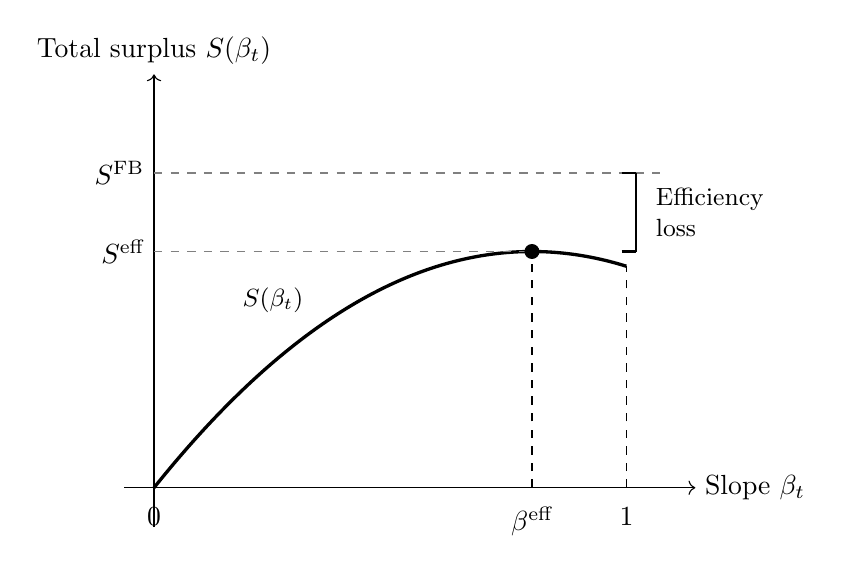
\begin{tikzpicture}[scale=1.25]
    \draw[->] (-0.3,0) -- (5.5,0) node[right] {Slope $\beta_t$};
    \draw[->] (0,-0.4) -- (0,4.2) node[above] {Total surplus $S(\beta_t)$};
    \draw[very thick, black, domain=0:4.8, smooth, variable=\x, samples=80]
        plot ({\x}, {6*(\x/4.8) - 3.75*(\x/4.8)^2});
    \draw[dashed, black] (3.84,0) -- (3.84,2.4);
    \node[below] at (3.84,-0.1) {$\beta^{\text{eff}}$};
    \draw[dashed, black] (4.8,0) -- (4.8,2.25);
    \node[below] at (4.8,-0.1) {$1$};
    \node[below] at (0,-0.1) {$0$};
    \draw[dashed, gray] (0,2.4) -- (3.84,2.4);
    \node[left] at (0,2.4) {$S^{\text{eff}}$};
    \draw[dashed, gray, thick] (0,3.2) -- (5.2,3.2);
    \node[left] at (0,3.2) {$S^{\text{FB}}$};
    \draw[thick, black] (4.9,2.4) -- (4.9,3.2);
    \draw[thick, black] (4.75,2.4) -- (4.9,2.4);
    \draw[thick, black] (4.75,3.2) -- (4.9,3.2);
    \node[right, font=\small, align=left] at (5.0, 2.8) {Efficiency\\loss};
    \filldraw[black] (3.84,2.4) circle (2pt);
    \node[right, font=\small] at (0.8,1.9) {$S(\beta_t)$};
\end{tikzpicture}
\caption*{Source: Own elaboration.}
\label{fig:surplus_curve}
\end{figure}
\vspace{-0.1cm}

%=======================================
\subsection{Nash bargaining solution}\label{subsec:nash}
%=======================================

In each period $t$, the principal and agent renegotiate the contract via Nash bargaining. Before agreement is reached, each party receives a disagreement payoff: $\overline{\Pi}$ for the principal and $\overline{\text{CE}}$ for the agent. These are exogenous outside options representing the payoffs available to each party if negotiations break down permanently. Their values are calibrated in Section \ref{subsec:calibration}.

The limited liability constraint requires that the agent's wage never falls below a minimum level that depends on her accumulated wealth $W_t$. We define this minimum level as
\[
\underline{w}_t = \overline{w} - \gamma_w W_t,
\]
where $\overline{w}$ is a baseline minimum wage and $\gamma_w \geq 0$ governs how the constraint relaxes with wealth. When $\gamma_w = 0$, limited liability is exogenous with a constant floor $\overline{w}$. When $\gamma_w > 0$, wealthier agents face less stringent constraints, consistent with wealth serving as collateral or commitment capacity. To ensure $w_t \geq \underline{w}_t$ holds for all output realizations under the linear contract $w_t = \alpha_t + \beta_t y_t$, we evaluate the constraint at the minimum possible output $\underline{y}$, the worst output realization the agent can produce. This gives $\alpha_t + \beta_t \underline{y} \geq \underline{w}_t$, or equivalently
\[
\alpha_t \geq \underline{w}_t - \beta_t \underline{y}.
\]

The agent's problem is governed by three standard constraints: incentive compatibility (IC), which ensures optimal effort choice; individual rationality (IR), which guarantees participation; and limited liability (LL), derived above. The Nash bargaining problem is
\[
\max_{(\alpha_t,\,\beta_t)\,\in\,\Gamma(W_t)} [\Pi_t - \overline{\Pi}]^{1-\delta} [\text{CE}_t - \overline{\text{CE}}]^{\delta},
\]
where $\delta \in (0,1)$ is the exogenous Nash bargaining parameter representing the agent's negotiating strength, and the feasible set is
\[
\Gamma(W_t) = \left\{(\alpha_t,\beta_t)\;\middle|\;
\underbrace{a_t^* = \tfrac{\beta_t\theta}{k}}_{\text{incentive compatibility (IC)}},\quad
\underbrace{\alpha_t \geq \underline{w}_t - \beta_t\,\underline{y}}_{\text{limited liability (LL)}},\quad
\underbrace{\Pi_t \geq \overline{\Pi},\;\text{CE}_t \geq \overline{\text{CE}}}_{\text{individual rationality (IR)}}
\right\}.
\]
The incentive compatibility constraint is already embedded in $\Pi_t$ and $\text{CE}_t$, which are written with optimal effort $a_t^* = \beta_t\theta/k$ substituted in. The individual rationality constraints are implicit in the domain of the Nash product, which is only defined when both parties weakly prefer agreement to disagreement. The substantive constraint is therefore limited liability, whose status determines the structure of the solution.

\paragraph{Case 1: Limited liability slack (unconstrained transfers).}

When transfers are unconstrained, $\alpha_t$ can be adjusted freely without affecting $\beta_t$ or total surplus. Since $\alpha_t$ enters $\text{CE}_t$ with coefficient $+1$ and $\Pi_t$ with coefficient $-1$, moving $\alpha_t$ by one unit transfers exactly one unit of surplus from the principal to the agent. The Pareto frontier in $(\Pi_t, \text{CE}_t)$ space is therefore a straight line with slope $-1$: any surplus division is achievable by adjusting $\alpha_t$ while keeping $\beta_t = \beta^{\text{eff}}$ fixed.

The first-order condition of the Nash product with respect to $\alpha_t$ gives
\[
\frac{1-\delta}{\Pi_t - \overline{\Pi}} = \frac{\delta}{\text{CE}_t - \overline{\text{CE}}}.
\]
Cross-multiplying and using $S_t = (\text{CE}_t - \overline{\text{CE}}) + (\Pi_t - \overline{\Pi})$, this implies
\[
(1-\delta)(\text{CE}_t - \overline{\text{CE}}) = \delta(\Pi_t - \overline{\Pi}),
\]
so that $\text{CE}_t - \overline{\text{CE}} = \delta S_t$ and $\Pi_t - \overline{\Pi} = (1-\delta)S_t$. Thus, the surplus split satisfies
\[
\frac{\text{CE}_t - \overline{\text{CE}}}{S_t} = \delta, \qquad \frac{\Pi_t - \overline{\Pi}}{S_t} = 1 - \delta,
\]
where each party receives exactly its Nash weight times total surplus.

Since $\alpha_t$ can be freely adjusted to split surplus, the Nash solution chooses $\beta_t = \beta^{\text{eff}}$ to maximize $S_t$, then sets $\alpha_t$ to deliver the agent a share $\delta$ of total surplus. Specifically,
\[
\alpha_t^* = \overline{\text{CE}} - C(\beta^{\text{eff}}) + \delta S(\beta^{\text{eff}}).
\]

This result is worth examining because, when limited liability is slack, realized bargaining power coincides exactly with the exogenous Nash parameter:
\[
\lambda_t := \frac{\text{CE}_t - \overline{\text{CE}}}{S_t} = \delta.
\]
The agent's share of surplus is pinned down by $\delta$ alone, regardless of wealth, history, or the level of output volatility. Bargaining power is truly exogenous in this regime: the linear frontier means that redistribution is costless, and the Nash solution simply picks the point on that line corresponding to weight $\delta$. This is the property that breaks down when limited liability binds.

\paragraph{Case 2: Limited liability binding (constrained transfers).}

When the limited liability constraint binds, $\alpha_t = \underline{w}_t - \beta_t \underline{y}$ and the fixed payment is no longer free: it is pinned by the constraint. Payoffs become functions of $\beta_t$ alone:
\[
\Pi_t(\beta_t) = D(\beta_t) + \beta_t \underline{y} - \underline{w}_t, \qquad \text{CE}_t(\beta_t) = C(\beta_t) - \beta_t \underline{y} + \underline{w}_t.
\]

To understand why the Pareto frontier is now curved, consider moving along it by changing $\beta_t$. Both $\Pi_t(\beta_t)$ and $\text{CE}_t(\beta_t)$ depend on $\beta_t$ through the functions $C(\beta_t)$ and $D(\beta_t)$, which are nonlinear. The slope of the frontier in $(\Pi_t, \text{CE}_t)$ space is
\[
\frac{d\,\text{CE}_t}{d\,\Pi_t} = \frac{\text{CE}_t'(\beta_t)}{\Pi_t'(\beta_t)},
\]
and the curvature is determined by the second derivative of $\text{CE}_t$ with respect to $\Pi_t$. Since $C(\beta_t)$ is concave and $D(\beta_t)$ is concave in $\beta_t$, the ratio $\text{CE}_t'(\beta_t)/\Pi_t'(\beta_t)$ is not constant: as $\beta_t$ increases, the marginal gain to one party differs from the marginal loss to the other, because both incentive provision and risk sharing respond nonlinearly to the slope. Formally, one can verify that $d^2\,\text{CE}_t / d\,\Pi_t^2 < 0$, so the frontier is strictly concave toward the origin. The economic content is that redistributing surplus in the binding regime is costly: changing $\beta_t$ to give more to the agent necessarily reduces total surplus, because $\beta_t$ is being asked to perform two tasks simultaneously, providing incentives and transferring resources, and it is not efficient at either task when pulled away from $\beta^{\text{eff}}$.

The Nash bargaining problem therefore reduces to a single-dimensional maximization:
\[
\max_{\beta_t} [\Pi_t(\beta_t) - \overline{\Pi}]^{1-\delta} [\text{CE}_t(\beta_t) - \overline{\text{CE}}]^{\delta}.
\]
This yields the first-order condition
\begin{equation}\label{eq:foc_binding}
(1-\delta) \frac{\Pi_t'(\beta_t^*)}{\Pi_t(\beta_t^*) - \overline{\Pi}} + \delta \frac{\text{CE}_t'(\beta_t^*)}{\text{CE}_t(\beta_t^*) - \overline{\text{CE}}} = 0,
\end{equation}
which implicitly defines the equilibrium slope $\beta_t^*$ as a function of wealth $W_t$ (through $\underline{w}_t$), disagreement payoffs $(\overline{\Pi}, \overline{\text{CE}})$, and the exogenous parameter $\delta$.

The agent's realized bargaining power is
\[
\lambda_t = \frac{\text{CE}_t(\beta_t^*) - \overline{\text{CE}}}{S_t(\beta_t^*)},
\]
where $S_t(\beta_t^*) = [\text{CE}_t(\beta_t^*) - \overline{\text{CE}}] + [\Pi_t(\beta_t^*) - \overline{\Pi}]$. Adjusting the surplus split requires changing $\beta_t$, which directly affects both risk sharing and incentive provision, so $S(\beta_t)$ varies with $\beta_t$ and the Pareto frontier is curved rather than linear, as illustrated in Figure \ref{fig:ntu_frontier}.

\begin{figure}[htbp]
\centering
\caption{Pareto frontiers in the slack (linear) and binding (curved) regimes. The linear frontier arises because $\alpha_t$ transfers surplus one-for-one between parties. The curved frontier arises because redistribution requires changing $\beta_t$, which affects total surplus nonlinearly. With the same Nash parameter $\delta$, the agent's realized share satisfies $\lambda^{\text{bind}} \neq \delta$ in the binding regime.}
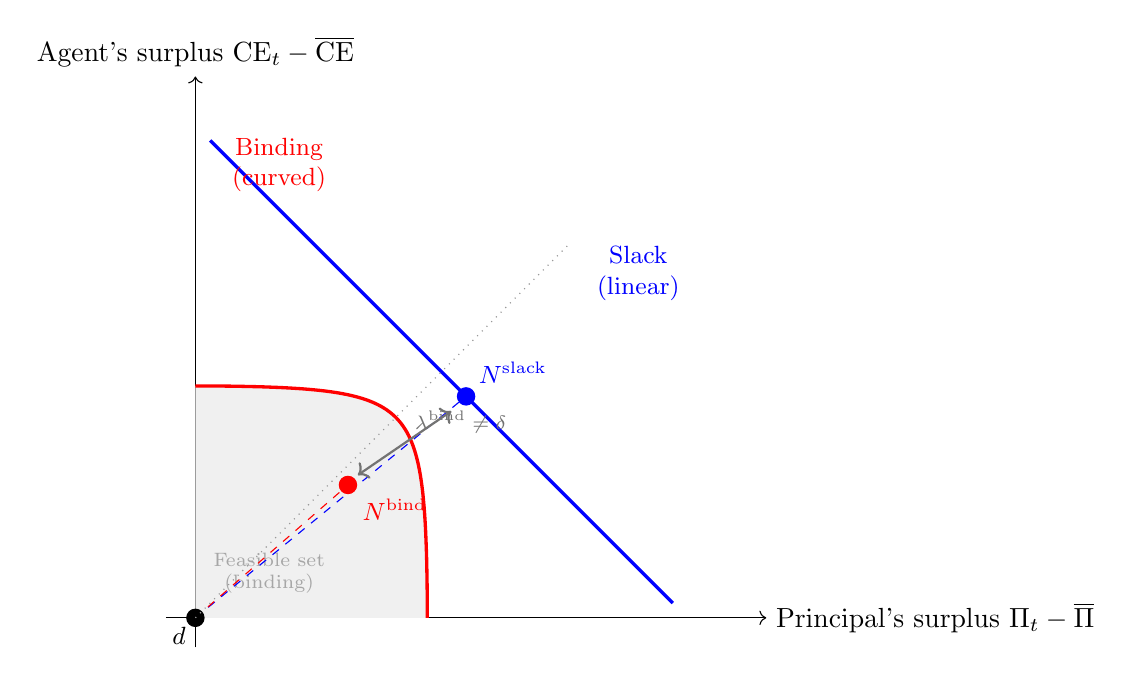
\begin{tikzpicture}[scale=1.25]
    \draw[->] (-0.3,0) -- (5.8,0) node[right] {Principal's surplus $\Pi_t - \overline{\Pi}$};
    \draw[->] (0,-0.3) -- (0,5.5) node[above] {Agent's surplus $\text{CE}_t - \overline{\text{CE}}$};

    \fill[gray!12] plot[domain=0:90, smooth, samples=60]
        ({3.8*sin(\x) * (1 - 0.38*sin(\x)^1.3)},
         {3.8*cos(\x) * (1 - 0.38*cos(\x)^1.3)})
        -- (0,0) -- cycle;
    \node[gray!70, font=\scriptsize, align=center] at (0.75,0.45) {Feasible set\\(binding)};

    \draw[very thick, blue] (0.15,4.85) -- (4.85,0.15);
    \node[blue, font=\small, align=center] at (4.5,3.5) {Slack\\(linear)};

    \filldraw[blue] (2.75,2.25) circle (2.5pt);
    \node[blue, font=\small, above right] at (2.78,2.28) {$N^{\text{slack}}$};
    \draw[dashed, blue, thin] (0,0) -- (2.75,2.25);

    \draw[very thick, red, domain=0:90, smooth, samples=80]
        plot ({3.8*sin(\x) * (1 - 0.38*sin(\x)^1.3)},
             {3.8*cos(\x) * (1 - 0.38*cos(\x)^1.3)});
    \node[red, font=\small, align=center] at (0.85,4.6) {Binding\\(curved)};

    \filldraw[red] (1.55,1.35) circle (2.5pt);
    \node[red, font=\small, right] at (1.6,1.1) {$N^{\text{bind}}$};
    \draw[dashed, red, thin] (0,0) -- (1.55,1.35);

    \filldraw[black] (0,0) circle (2.5pt);
    \node[below left, font=\small] at (0,0) {$d$};

    \draw[<->, thick, black!55] (2.6,2.1) -- (1.65,1.45)
        node[midway, above right, font=\scriptsize] {$\lambda^{\text{bind}} \neq \delta$};

    \draw[dotted, black!40, thin] (0,0) -- (3.8,3.8);

\end{tikzpicture}
\caption*{\text{Source:} Own elaboration.}
\label{fig:ntu_frontier}
\end{figure}

Since $\underline{w}_t$ depends on wealth through $W_t$, and $\beta_t^*$ depends on $\underline{w}_t$, realized bargaining power $\lambda_t$ becomes history-dependent through the wealth accumulation process. In general, $\lambda_t \neq \delta$ when the constraint binds. When limited liability does not bind, the Pareto frontier is linear and the Nash solution achieves any surplus split by adjusting $\alpha_t$ while keeping efficiency at $\beta^{\text{eff}}$, so $\lambda_t = \delta$ always. When limited liability binds, the constraint pins $\alpha_t$ and the Pareto frontier becomes curved: points corresponding to different wealth levels face different feasible sets, so their realized bargaining power differs even under the same exogenous Nash parameter $\delta$. Moving along the curved frontier requires changing $\beta_t$, which affects total surplus and generates the non-transferability that makes bargaining outcomes history-dependent.

\begin{remark}[Welfare comparison: constrained planner versus Nash equilibrium]\label{rem:welfare}
The binding regime generates a third layer of efficiency loss, on top of the two already identified in Section \ref{subsec:symmetric}. To see this, consider a constrained planner who respects incentive compatibility and limited liability but is not subject to Nash bargaining: the planner maximizes total surplus $S(\beta)$ subject to $\alpha \geq \underline{w}(W) - \beta\underline{y}$.

The planner sets $\alpha = \underline{w}(W) - \beta\underline{y}$ at the boundary (since any slacker $\alpha$ wastes surplus), but is free to choose $\beta$ independently to maximize $S(\beta)$. The limited liability constraint binds only on $\alpha$, not on $\beta$. The planner therefore implements $\beta^{\mathrm{eff}}$ regardless of $W$, achieving $S^{\mathrm{eff}} = S(\beta^{\mathrm{eff}})$ in every period.

The Nash equilibrium in the binding regime instead chooses $\beta^*(W) \neq \beta^{\mathrm{eff}}$, because the parties use $\beta_t$ both to set incentives and to redistribute surplus. The resulting equilibrium surplus is $S(\beta^*(W)) < S(\beta^{\mathrm{eff}})$, since $\beta^{\mathrm{eff}}$ is the unique maximizer of $S(\beta)$. The bargaining distortion is
\[
\Delta(W) := S^{\mathrm{eff}} - S(\beta^*(W)) = \frac{(\beta^{\mathrm{eff}} - \beta^*(W))^2}{2} \left(\frac{\theta^2}{k} + \gamma\sigma^2\right) > 0,
\]
where the equality uses the quadratic form of $S(\beta)$ around its maximum. Three features of $\Delta(W)$ are worth noting. First, $\Delta(W) = 0$ in the slack regime, where $\beta^*(W) = \beta^{\mathrm{eff}}$: bargaining introduces no additional distortion when transfers are unconstrained. Second, $\Delta(W)$ is increasing in $|\beta^*(W) - \beta^{\mathrm{eff}}|$, which is itself increasing in how far $W$ is below $\overline{W}$: poorer agents face tighter constraints, larger distortions in $\beta^*$, and greater welfare losses. Third, $\Delta(W)$ is increasing in $\theta^2/k + \gamma\sigma^2$, the curvature of the surplus function: when the risk-incentive trade-off is steep, small deviations of $\beta^*$ from $\beta^{\mathrm{eff}}$ are more costly.

The full efficiency loss relative to first-best therefore decomposes as
\[
S^{\mathrm{FB}} - S(\beta^*(W)) = \underbrace{(S^{\mathrm{FB}} - S^{\mathrm{eff}})}_{\text{moral hazard}} + \underbrace{\Delta(W)}_{\text{bargaining distortion}},
\]
with the second term present only in the binding regime and vanishing as $W \to \overline{W}$. This decomposition clarifies that policies reducing the stringency of the limited liability constraint (raising $\gamma_w$ or increasing $W$) improve welfare not only by relaxing the constraint directly but also by reducing the bargaining distortion $\Delta(W)$.
\end{remark}

%=======================================
\subsection{Dynamic environment and recursive formulation}\label{subsec:dynamics}
%=======================================

We now embed the contracting problem in a dynamic environment. Time is discrete, indexed by $t=0,1,2,\dots$. In each period, after observing the current public state, the principal and the agent renegotiate a one-period contract through Nash bargaining, taking into account its effect on future continuation values.

The key state variable is the agent's accumulated wealth $W_t$. Unlike the formulation of \textcite{spear1987}, where the agent's promised discounted utility serves as the sufficient state variable, here accumulated wealth plays that role because the wealth-dependent limited liability constraint ties feasibility directly to $W_t$. A full justification of this reduction appears later in this subsection. We assume that wealth is publicly observable. This assumption is essential for the recursive formulation. At the end of each period, output $y_t$ and the agreed contract $(\alpha_t,\beta_t)$ are publicly observed. Since under incentive compatibility effort is pinned down by the contract through
\[
a_t^*=\frac{\beta_t\theta}{k},
\]
both parties can infer the realized transfer and update wealth according to
\[
W_{t+1}=W_t+\alpha_t+\beta_t y_t-\frac{k}{2}(a_t^*)^2.
\]
Therefore, the next-period limited liability threshold
\[
\underline{w}(W_{t+1})=\overline w-\gamma_w W_{t+1}
\]
is common knowledge at the start of period $t+1$.

In general, an infinitely repeated contracting problem is not stationary \parencite[see][section~2]{spear1987}: the optimal contract at date $t$ may depend on the entire past history $h^t = (y_0, \alpha_0, \beta_0, \dots, y_{t-1}, \alpha_{t-1}, \beta_{t-1})$, making a direct recursive characterization unavailable. \textcite{spear1987} resolve this difficulty in the standard repeated moral hazard problem by demonstrating that the agent's promised discounted utility serves as a sufficient state variable: conditioning on it, no additional history is needed to describe the optimal continuation contract. Their argument proceeds by showing that any optimal contract is completely characterized by four stationary functions, a compensation schedule, a continuation value rule, a policy function for effort, and a value function for the principal, satisfying regeneration conditions, so that the infinite-horizon problem reduces to a static variational problem parametrized by the promised utility level.

We now carry out the analogous reduction in our setting, establishing that accumulated wealth $W_t$ plays the role that promised utility plays in \textcite{spear1987}.

Let $\{(\alpha_t, \beta_t)\}_{t \geq 0}$ be an optimal contract. For any date $t$ and history $h^t$, let $W_t = W_t(h^t)$ denote the resulting wealth and let $V_P(h^t)$ and $V_A(h^t)$ denote the principal's and agent's continuation values from period $t$ onward. We claim that these continuation values depend on $h^t$ only through $W_t$.

\textit{Dominance argument.} Suppose, toward a contradiction, that at two histories $h^t$ and $\tilde{h}^t$ satisfying $W_t(h^t) = W_t(\tilde{h}^t) = W$, the optimal continuation contract at $\tilde{h}^t$ achieves a strictly higher principal payoff while delivering the agent the same continuation utility as the optimal continuation at $h^t$. Then the contract that follows the plan for $h^t$ through date $t$ and switches to the $\tilde{h}^t$ continuation from period $t+1$ onward is feasible and yields the principal a strictly higher payoff, contradicting optimality of the original contract. The argument requires verifying that switching continuation plans at the same $W_t$ is indeed feasible regardless of the path that generated it.

\textit{Why $W_t$ is a sufficient statistic.} Two structural properties of the model ensure that every constraint a continuation contract must satisfy at state $W$ depends on history only through $W$.

First, because contracts are linear and the agent's utility is CARA with coefficient $\gamma$, the agent's certainty equivalent at any period is
\[
\mathrm{CE}_t(\alpha_t, \beta_t) = \alpha_t + C(\beta_t),
\]
where $C(\beta_t) = \beta_t^2\theta^2/(2k) - (\gamma/2)\beta_t^2\sigma^2$ depends only on the current contract parameters. The discounted expected utility the agent derives from a continuation plan starting from wealth $W$ is therefore additive in $W$: shifting $W$ up by one unit shifts the reachable fixed payments $\alpha_{t+s}$ by $\gamma_w$ for all $s \geq 1$ through the limited liability threshold, which translates into an additive shift in the certainty equivalent at each future date. This additive separability means that two histories sharing the same $W_t$ give rise to payoff-equivalent continuation problems. It is the CARA-linear contract structure that delivers this property; without it, the certainty equivalent would depend on the full path of past wages and wealth, not just the current stock.

Second, the limited liability threshold $\underline{w}(W_t) = \overline{w} - \gamma_w W_t$ is the only channel through which history enters the feasibility constraint on the continuation contract. Because $W_t$ fully determines this threshold, two paths leading to the same $W_t$ generate exactly the same feasible set $\Gamma(W_t)$ of continuation contracts. No further knowledge of past outputs or transfers is required.

Together, these two properties imply that $W_t$ summarizes all payoff-relevant history for the continuation problem. The dominance argument then goes through: any continuation contract achievable at $\tilde{h}^t$ with wealth $W$ is equally achievable at $h^t$ with the same wealth, so the optimal continuation value at any state $W$ is uniquely defined regardless of path.

The reduction above implies that the optimal contract from any state $W$ is completely characterized by four stationary functions: a compensation intercept $\alpha^*(W)$, an incentive slope $\beta^*(W)$, a principal value function $V_P(W)$, and an agent value function $V_A(W)$. These functions must satisfy the following regeneration conditions, which are the direct analogues of conditions (ii) and (iii) in \textcite{spear1987}. For all $W$ in the equilibrium domain, with $W' = W + \alpha^*(W) + \beta^*(W)y - \frac{k}{2}(a^*(\beta^*(W)))^2$ and $y = \theta a^* + \sigma\varepsilon$, $\varepsilon \sim \mathcal{N}(0,1)$:
\begin{align}
V_P(W) &= \Pi(\alpha^*(W), \beta^*(W)) + \rho\,\mathbb{E}\bigl[V_P(W') \mid W\bigr], \label{eq:regen_P} \\
V_A(W) &= \mathrm{CE}(\alpha^*(W), \beta^*(W)) + \rho\,\mathbb{E}\bigl[V_A(W') \mid W\bigr]. \label{eq:regen_A}
\end{align}
Equation \eqref{eq:regen_P} requires that $V_P(W)$ is the payoff the principal actually receives when the stationary policy is followed from state $W$. Equation \eqref{eq:regen_A} imposes the same consistency for the agent. Given these functions, the infinite-horizon problem reduces to choosing $(\alpha^*(\cdot), \beta^*(\cdot), V_P(\cdot), V_A(\cdot))$ to solve the Nash bargaining problem at each $W$, subject to feasibility, incentive compatibility, limited liability, and the regeneration conditions \eqref{eq:regen_P}-\eqref{eq:regen_A}. This is the static variational problem in the sense of \textcite{spear1987}, now parametrized by wealth rather than promised utility.

The key distinction from \textcite{spear1987} is the identity of the state variable. In their formulation, the agent's promised utility $w_t$ is the state variable because it summarizes the history of incentive-compatible continuation promises. In our formulation, accumulated wealth $W_t$ plays this role because it summarizes the history of constrained transfers through the limited liability channel. The two representations are connected: under binding limited liability, higher promised utility corresponds to greater accumulated wealth, since a wealthier agent faces a less stringent floor and can be promised a larger certainty equivalent. Our formulation makes this connection explicit and derives the state-variable role of wealth from primitives.

For a given state $W$, a feasible contract $(\alpha,\beta)$ must satisfy:
\begin{enumerate}
    \item incentive compatibility: $a^*(\beta)=\beta\theta/k$;
    \item limited liability: $\alpha \geq \underline{w}(W)-\beta \underline y$, where $\underline y$ denotes the lower bound of output support.\footnote{The analysis in this section is written for a setting in which output has lower-bounded support. This can be interpreted either literally, by assuming bounded shocks, or as a tractable approximation to the Gaussian benchmark used above. What matters for the mechanism is that binding limited liability places a lower bound on feasible transfers.}
\end{enumerate}

Given a feasible contract $(\alpha,\beta)$, current payoffs are $\Pi(\alpha,\beta)=D(\beta)-\alpha$ and $\mathrm{CE}(\alpha,\beta)=\alpha+C(\beta)$, where $C(\beta)$ and $D(\beta)$ are as defined in Section \ref{subsec:moral_hazard}, and next-period wealth is
\[
W' = W+\alpha+\beta y-\frac{k}{2}(a^*(\beta))^2,\qquad y=\theta a^*(\beta)+\sigma \varepsilon,\qquad\varepsilon\sim \mathcal N(0,1).
\]

Let $V_P(W)$ and $V_A(W)$ denote the principal's and agent's equilibrium continuation values when the current public state is $W$. If agreement is not reached, the relationship breaks down and the parties receive exogenous outside options $\overline{\Pi}$ and $\overline{\text{CE}}$, respectively.

The formulation is recursive because rather than specifying an optimal contract as a sequence indexed by $t$, we look for stationary functions $\alpha^*(\cdot)$ and $\beta^*(\cdot)$ that solve the same problem at every state $W$. This makes the infinite-horizon problem tractable: once the value functions $V_P$ and $V_A$ are known, the optimal contract at any date follows from evaluating those stationary functions at the current state.

\begin{definition}[Recursive Nash bargaining problem]\label{def:recursive_nash}
Given current public wealth $W$, the recursive Nash bargaining problem is
\[
(\alpha^*(W),\beta^*(W))
\in
\arg\max_{(\alpha,\beta)\in\Gamma(W)}
\Big[V_P^{c}(W;\alpha,\beta)-\overline{\Pi}\Big]^{1-\delta}
\Big[V_A^{c}(W;\alpha,\beta)-\overline{\text{CE}}\Big]^{\delta},
\]
where $\Gamma(W)$ is the set of feasible contracts at state $W$, and
\begin{align*}
    V_P^{c}(W;\alpha,\beta)&=\Pi(\alpha,\beta)+\rho\,\mathbb E\big[V_P(W')\mid W,\alpha,\beta\big],\\
    V_A^{c}(W;\alpha,\beta)&=\mathrm{CE}(\alpha,\beta)+\rho\,\mathbb E\big[V_A(W')\mid W,\alpha,\beta\big].
\end{align*}
\end{definition}

The recursive structure of Definition \ref{def:recursive_nash} is visible in the continuation terms $\rho\,\mathbb{E}[V_P(W')\mid W,\alpha,\beta]$ and $\rho\,\mathbb{E}[V_A(W')\mid W,\alpha,\beta]$: the value functions $V_P$ and $V_A$ appear in the objective today and are evaluated at the next-period state $W'$ that results from today's contract. The same functions that define what the parties bargain over today govern their continuation payoffs tomorrow.

Definition \ref{def:recursive_nash} makes explicit that the contract chosen today affects future bargaining through the law of motion of wealth. The problem is inherently dynamic: current allocations affect not only contemporaneous payoffs but also future feasibility through the evolution of wealth.

\begin{remark}[Timing and renegotiation-proofness]\label{rem:renegotiation}
The stage game within each period $t$ follows a specific timing that makes within-period renegotiation infeasible. At the start of period $t$, the public state $W_t$ is observed. The principal and agent bargain over the one-period contract $(\alpha_t, \beta_t)$. Once agreement is reached, the agent chooses effort $a_t^* = \beta_t\theta/k$, output $y_t$ is realized, the transfer $w_t = \alpha_t + \beta_t y_t$ is paid, and wealth $W_{t+1}$ is updated. Because the contract is agreed upon before effort is chosen and before output is realized, neither party can condition a within-period renegotiation offer on the effort choice or on the output realization.

Two features of the equilibrium then rule out profitable within-period renegotiation. In the slack regime, the perfect Markov stationary equilibrium (PMSE, defined formally in Definition~\ref{def:pmse} below) contract implements the efficient slope $\beta^{\mathrm{eff}}$ and splits surplus according to $\delta$; any alternative contract would move the parties off the Pareto frontier. In the binding regime, the PMSE contract is the unique maximizer of the Nash product on $\Gamma(W_t)$ (Proposition \ref{prop:existence}); any alternative contract $(\alpha_t', \beta_t')$ that both parties weakly prefer would also have to lie in $\Gamma(W_t)$, contradicting the uniqueness of the Nash solution.

This argument does not rule out renegotiation at the start of period $t+1$, before a new contract is drawn. That renegotiation is precisely what Definition \ref{def:recursive_nash} models: the parties re-optimize given $W_{t+1}$. The PMSE is therefore an equilibrium of a game in which the contract is fully renegotiated each period, with each period's negotiation history-dependent through $W_t$ via the limited liability channel.
\end{remark}


The regeneration conditions \eqref{eq:regen_P}-\eqref{eq:regen_A} can be stated compactly as a pair of coupled Bellman equations. Because the equilibrium is stationary, these equations are written in terms of value functions of the state $W$ alone, without an explicit time index; the index $t$ appears only through the law of motion of $W$ when the equations are iterated forward. Let $\mathcal{S} \subseteq \mathbb{R}$ denote the compact equilibrium wealth domain defined formally in Assumption \ref{ass:compact_domain}, and let $C(\mathcal{S})$ denote the Banach space of continuous bounded functions on $\mathcal{S}$ equipped with the supremum norm $\|f\|_\infty = \sup_{W \in \mathcal{S}} |f(W)|$. Define the operator $T = (T_P, T_A)$ acting on pairs $(V_P, V_A) \in C(\mathcal{S}) \times C(\mathcal{S})$ by
\begin{align}
    T_P V_P(W) &:= \Pi\!\bigl(\alpha^*(W),\beta^*(W)\bigr)
    + \rho\,\mathbb{E}\bigl[V_P(W') \mid W, \alpha^*(W), \beta^*(W)\bigr],
    \label{eq:bellman_P}\\[4pt]
    T_A V_A(W) &:= \mathrm{CE}\!\bigl(\alpha^*(W),\beta^*(W)\bigr)
    + \rho\,\mathbb{E}\bigl[V_A(W') \mid W, \alpha^*(W), \beta^*(W)\bigr],
    \label{eq:bellman_A}
\end{align}
where $(\alpha^*(W),\beta^*(W))$ is the contract solving the recursive Nash bargaining problem in Definition \ref{def:recursive_nash} given the current value functions, and $W'$ follows the law of motion under that contract. A stationary equilibrium is a fixed point of $T$: a pair $(V_P^*, V_A^*)$ satisfying $T_P V_P^* = V_P^*$ and $T_A V_A^* = V_A^*$ simultaneously. Proposition \ref{prop:existence} establishes that $T$ is a contraction of modulus $\rho$ on $C(\mathcal{S}) \times C(\mathcal{S})$, so the Contraction Mapping Theorem delivers the unique fixed point.

%=======================================
\subsection{Perfect Markov stationary equilibrium}\label{subsec:pmse}
%=======================================

We focus on equilibria in which strategies depend only on current wealth and are time-invariant.

\begin{definition}[Perfect Markov Stationary Equilibrium]\label{def:pmse}
A Perfect Markov Stationary Equilibrium (PMSE) \parencite{maskin1994, fudenberg1991} is a collection of value functions $(V_P,V_A)$ and policy functions $(\alpha^*,\beta^*)$ such that, for every $W$ in the equilibrium domain:
\begin{enumerate}
    \item \textit{Markov property}: $(\alpha^*(W),\beta^*(W))$ depends only on current wealth $W$;
    \item \textit{Stationarity}: the same policy functions apply at every date;
    \item \textit{Optimality}: $(\alpha^*(W),\beta^*(W))$ solves the recursive Nash bargaining problem in Definition \ref{def:recursive_nash};
    \item \textit{Consistency}: the continuation values satisfy $V_P(W)=V_P^{c}(W;\alpha^*(W),\beta^*(W))$ and $V_A(W)=V_A^{c}(W;\alpha^*(W),\beta^*(W))$.
\end{enumerate}
\end{definition}

The PMSE concept is appropriate here because wealth is publicly observable and payoff-relevant only through its effect on the limited liability threshold. Conditional on $W_t$, past realizations matter only insofar as they are summarized by current wealth. Hence no additional history is needed to describe equilibrium behavior, which is what makes recursive methods applicable \parencite{stokey1989}.

To state the existence result precisely, we first collect the domain assumptions in a single place.

\begin{assumption}[Compact equilibrium domain]\label{ass:compact_domain}
Fix parameters $(\theta, k, \gamma, \sigma, \rho, \delta, \overline{w}, \gamma_w, \underline{y})$ satisfying $\gamma_w < 1$. Define $\mathcal{S} := [\underline{W}, W_{\max}]$ where $\underline{W}$ is the lower boundary of the binding regime and $W_{\max} < \infty$ is chosen large enough that the ergodic support of $\{W_t\}$ is contained in $\mathcal{S}$, as guaranteed by Proposition \ref{prop:ergodic}. On this domain:
\begin{enumerate}
    \item The feasible correspondence $\Gamma : \mathcal{S} \rightrightarrows [0,1]$ is nonempty, compact-valued, and continuous.
    \item Period payoffs $\Pi(\alpha,\beta)$ and $\mathrm{CE}(\alpha,\beta)$ are continuous and bounded on $\mathcal{S} \times [0,1]$.
    \item The Nash product $[\Pi(\alpha,\beta) - \overline{\Pi}]^{1-\delta}[\mathrm{CE}(\alpha,\beta) - \overline{\text{CE}}]^{\delta}$ is strictly quasiconcave in $(\alpha,\beta)$ on $\Gamma(W)$ for every $W \in \mathcal{S}$.
\end{enumerate}
\end{assumption}

Parts (1) and (2) hold because $\Gamma(W)$ is defined by linear constraints in $(\alpha,\beta)$ with coefficients continuous in $W$, and period payoffs are polynomial in $(\alpha,\beta)$ hence continuous and bounded on the compact set $\mathcal{S} \times [0,1]$. Part (3) follows from the single-crossing property of the Nash first-order condition established in Lemma \ref{lem:beta_bounds}: $F(\beta, W)$ changes sign exactly once from positive to negative on $(0,1)$, which is equivalent to the Nash product having a unique interior maximizer.

\begin{proposition}[Existence and uniqueness of stationary equilibrium]\label{prop:existence}
Under Assumption \ref{ass:compact_domain}, there exist unique continuous value functions $V_P^*, V_A^* \in C(\mathcal{S})$ and unique measurable policy functions $\alpha^* : \mathcal{S} \to \mathbb{R}$, $\beta^* : \mathcal{S} \to [0,1]$ constituting a PMSE.
\end{proposition}

\begin{proof}
Define Bellman operators $T_P, T_A : C(\mathcal{S}) \to C(\mathcal{S})$ by
\begin{align}
T_P V_P(W) &:= \Pi(\alpha^*(W),\beta^*(W)) + \rho\,\mathbb{E}\bigl[V_P(W') \mid W, \alpha^*(W), \beta^*(W)\bigr], \label{eq:proof_TP} \\
T_A V_A(W) &:= \mathrm{CE}(\alpha^*(W),\beta^*(W)) + \rho\,\mathbb{E}\bigl[V_A(W') \mid W, \alpha^*(W), \beta^*(W)\bigr], \label{eq:proof_TA}
\end{align}
where $(\alpha^*(W),\beta^*(W))$ denotes the maximizer of the Nash product in Definition \ref{def:recursive_nash} given the current value functions. Let $T := (T_P, T_A)$ act on the product space $C(\mathcal{S}) \times C(\mathcal{S})$ equipped with the sup norm $\|(V_P, V_A)\|_\infty := \max(\|V_P\|_\infty, \|V_A\|_\infty)$.

We verify Blackwell's sufficient conditions for $T$ to be a contraction \parencite[Theorem 3.3]{stokey1989}.

\textit{Monotonicity.} If $V_P \leq \tilde{V}_P$ pointwise on $\mathcal{S}$, then for every feasible contract $(\alpha,\beta)$,
\[
\mathbb{E}[V_P(W') \mid W, \alpha, \beta] \leq \mathbb{E}[\tilde{V}_P(W') \mid W, \alpha, \beta],
\]
so $T_P V_P(W) \leq T_P \tilde{V}_P(W)$ for every $W \in \mathcal{S}$. The argument for $T_A$ is identical.

\textit{Discounting.} For any constant $c \geq 0$ and any $V_P \in C(\mathcal{S})$,
\[
T_P(V_P + c)(W) = \Pi(\alpha^*,\beta^*) + \rho\,\mathbb{E}[V_P(W') + c \mid W, \alpha^*,\beta^*] = T_P V_P(W) + \rho c,
\]
since $c$ is constant and the maximizing contract is unchanged. Hence $T$ satisfies the discounting condition with modulus $\rho \in (0,1)$.

By Blackwell's theorem, $T$ is a contraction of modulus $\rho$ on the complete metric space $C(\mathcal{S}) \times C(\mathcal{S})$. The Contraction Mapping Theorem \parencite[Theorem 3.2]{stokey1989} yields a unique fixed point $(V_P^*, V_A^*)$, with $T_P V_P^* = V_P^*$ and $T_A V_A^* = V_A^*$. These are the regeneration conditions \eqref{eq:regen_P}-\eqref{eq:regen_A}.

\textit{Continuity of value functions.} Since payoffs and the transition kernel are continuous in $W$ on $\mathcal{S}$ (Assumption \ref{ass:compact_domain}), an induction argument shows that $T^n V_P \in C(\mathcal{S})$ for any $V_P \in C(\mathcal{S})$ and all $n \geq 1$. Because $C(\mathcal{S})$ is closed under the contraction limit, $V_P^* \in C(\mathcal{S})$.

\textit{Policy functions.} The feasible correspondence $\Gamma(W)$ is compact-valued and continuous by Assumption \ref{ass:compact_domain}. The Nash product is continuous in $(\alpha,\beta,W)$ and strictly quasiconcave in $(\alpha,\beta)$ on $\Gamma(W)$ for every $W$. Berge's Maximum Theorem implies the value of the Nash problem is continuous in $W$ and the policy correspondence is upper hemicontinuous. Strict quasiconcavity implies the maximizer is unique at each $W$, so the correspondence reduces to a function. The resulting $\alpha^*(\cdot)$ and $\beta^*(\cdot)$ are therefore measurable selections, and by continuity of the Nash product and compactness of $\Gamma(W)$, they are in fact continuous.

The collection $(V_P^*, V_A^*, \alpha^*, \beta^*)$ satisfies all four conditions of Definition \ref{def:pmse} by construction.
\end{proof}

\begin{remark}[Uniqueness of policy functions]
Uniqueness of $(V_P^*, V_A^*)$ follows from the Contraction Mapping Theorem. Uniqueness of $(\alpha^*, \beta^*)$ is a separate statement: it follows from strict quasiconcavity of the Nash product (Assumption \ref{ass:compact_domain}, Part 3), which rules out multiple maximizers at any $W \in \mathcal{S}$.
\end{remark}

Proposition \ref{prop:existence} establishes that the model admits a recursive stationary representation with unique value and policy functions on the equilibrium domain. In what follows, we characterize the equilibrium more sharply in the two regimes generated by limited liability.

%=======================================
\subsection{Binding regime and reduced recursive representation}\label{subsec:binding_dynamic}
%=======================================

When limited liability is slack, $\alpha$ remains a pure transfer and the Nash solution selects the efficient slope $\beta^{\mathrm{eff}}$ and uses $\alpha$ to split continuation surplus according to $\delta$. This follows from the slack-regime characterization in Proposition \ref{prop:tu_ntu}: when the constraint does not bind, the feasible set $\Gamma(W)$ is unconstrained in $\alpha$, so the Pareto frontier is linear and the Nash solution recovers the standard split.

The mechanism of interest arises when limited liability binds. In that regime, $\alpha = \underline{w}(W)-\beta \underline y$, so the fixed payment is no longer a free transfer but is pinned by the constraint, so the bargaining problem reduces to a choice over $\beta$ alone. Substituting the binding constraint into Definition \ref{def:recursive_nash}, continuation values become
\[
V_P^{b}(W;\beta)=D(\beta)+\beta \underline y-\underline{w}(W)+\rho\,\mathbb E\big[V_P(W')\mid W,\beta\big],
\]
\[
V_A^{b}(W;\beta)=C(\beta)-\beta \underline y+\underline{w}(W)+\rho\,\mathbb E\big[V_A(W')\mid W,\beta\big].
\]

The state-dependent Nash problem in the binding regime is therefore
\[
\beta^*(W)\in\arg\max_{\beta\in[0,1]}
\Big[V_P^{b}(W;\beta)-\overline{\Pi}\Big]^{1-\delta}
\Big[V_A^{b}(W;\beta)-\overline{\text{CE}}\Big]^{\delta},
\]
with first-order condition
\begin{equation}\label{eq:foc_binding_dynamic}
(1-\delta)\frac{\dfrac{\partial V_P^{b}}{\partial\beta}(W;\beta^*)}{V_P^{b}(W;\beta^*)-\overline{\Pi}}
+
\delta\,\frac{\dfrac{\partial V_A^{b}}{\partial\beta}(W;\beta^*)}{V_A^{b}(W;\beta^*)-\overline{\text{CE}}}
=0.
\end{equation}

Equation \eqref{eq:foc_binding_dynamic} is the dynamic analogue of the static binding-regime condition \eqref{eq:foc_binding}. When continuation values are linear in current payoffs, as in the static benchmark, \eqref{eq:foc_binding_dynamic} reduces exactly to \eqref{eq:foc_binding}, with $\Pi$ and $\mathrm{CE}$ replacing $V_P^b$ and $V_A^b$. In the general dynamic case, the equilibrium slope must additionally account for how changing $\beta$ shifts next-period wealth and therefore next-period feasibility.

The agent's realized bargaining power in the binding regime is defined as the agent's share of total equilibrium surplus:
\[
\lambda(W)=\frac{V_A^{b}(W;\beta^*(W))-\overline{\text{CE}}}{\big[V_P^{b}(W;\beta^*(W))-\overline{\Pi}\big]+\big[V_A^{b}(W;\beta^*(W))-\overline{\text{CE}}\big]}.
\]
The formula itself is the standard definition of the agent's surplus share in any Nash bargaining problem. What is specific to this model is that $\lambda(W)$ is not pinned down by the exogenous weight $\delta$ but is determined by the equilibrium contract $\beta^*(W)$, which depends on wealth through the binding limited liability constraint.
Unlike in the slack regime, $\lambda(W)$ need not coincide with $\delta$, because changing the surplus split now requires changing $\beta$, and this affects total surplus itself.

%=======================================
\subsection{Equilibrium properties and endogenous bargaining dynamics}\label{subsec:equilibrium}
%=======================================

\begin{figure}[htbp]
\centering
\caption{Schematic representation of the endogenous bargaining power mechanism.}
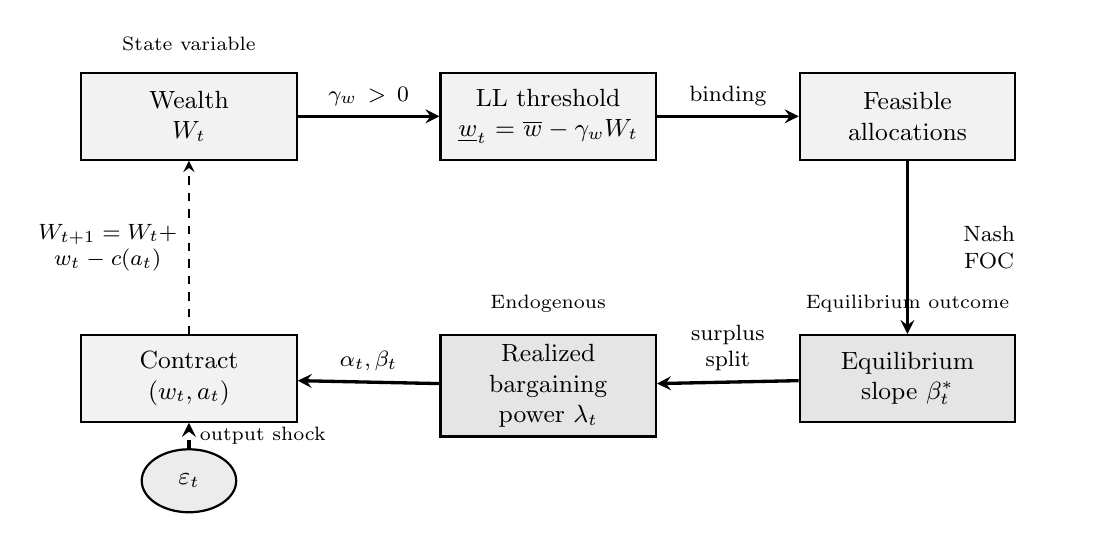
\begin{tikzpicture}[
    node distance=2.2cm and 1.8cm,
    box/.style={rectangle, draw, thick, text width=2.5cm, align=center, minimum height=1.1cm, font=\small},
    arrow/.style={->, >=stealth, very thick},
    label/.style={font=\footnotesize, text width=1.8cm, align=center}
]
    \node[box, fill=gray!10] (wealth) {Wealth\\$W_t$};
    \node[box, fill=gray!10, right=of wealth] (constraint) {LL threshold\\$\underline{w}_t = \overline{w} - \gamma_w W_t$};
    \node[box, fill=gray!10, right=of constraint] (feasible) {Feasible\\allocations};
    
    \node[box, fill=gray!10, below=of wealth] (contract) {Contract\\$(w_t, a_t)$};
    \node[box, fill=gray!20, below=of constraint] (lambda) {Realized\\bargaining\\power $\lambda_t$};
    \node[box, fill=gray!20, below=of feasible] (beta) {Equilibrium\\slope $\beta_t^*$};
    
    \draw[arrow, black] (wealth) -- (constraint) node[midway, above, label] {$\gamma_w > 0$};
    \draw[arrow, black] (constraint) -- (feasible) node[midway, above, label] {binding};
    \draw[arrow, black] (feasible) -- (beta) node[midway, right, label] {Nash\\FOC};
    \draw[arrow, black] (beta) -- (lambda) node[midway, above, label] {surplus\\split};
    \draw[arrow, black] (lambda) 
    -- (contract) node[midway, above, label] {$\alpha_t, \beta_t$};
    
    \draw[arrow, black, dashed, thick] (contract) -- (wealth) node[midway, left, label] {$W_{t+1} = W_t +$\\$w_t - c(a_t)$};
    
    \node[draw, ellipse, thick, fill=gray!15, minimum width=1.2cm, minimum height=0.8cm, font=\small] at ($(contract) + (0, -1.3)$) (shock) {$\varepsilon_t$};
    \draw[arrow, dashed] (shock) -- (contract) node[midway, right, font=\scriptsize] {output shock};
    
    \node[above=0.15cm of wealth, font=\scriptsize, text=black] {State variable};
    \node[above=0.15cm of beta, font=\scriptsize, text=black] {Equilibrium outcome};
    \node[above=0.15cm of lambda, font=\scriptsize, text=black] {Endogenous};
    
\end{tikzpicture}
\caption*{\text{Source:} Own elaboration.}
\label{fig:mechanism}
\end{figure}

Figure \ref{fig:mechanism} provides a schematic overview of the feedback mechanism that generates endogenous bargaining power evolution. Wealth $W_t$ determines the limited liability threshold $\underline{w}_t$ through the parameter $\gamma_w$. When this constraint binds, it restricts the feasible allocation set. The Nash bargaining solution then determines an equilibrium slope $\beta_t^*$, which in turn determines realized bargaining power $\lambda_t$ through the implied surplus split. The resulting contract generates next period's wealth through the budget constraint, with random shocks $\varepsilon_t$ to output creating persistence in bargaining outcomes. The responsiveness of bargaining power to shocks, characterized in Proposition \ref{prop:dynamics}, is proportional to $\beta_t^*\sigma$, with the role of $\gamma_w$ entering through the sensitivity of $\lambda(W_t)$ to wealth.

The feedback loop depicted in Figure \ref{fig:mechanism} admits a precise characterization. Before stating the supporting results, we collect the central claim of the paper in a single theorem.

\begin{theorem}[Limited liability and endogenous bargaining power] \label{thm:central}
When the limited liability floor is wealth-dependent with $\gamma_w > 0$, binding limited liability transforms realized bargaining power from a fixed primitive into a state variable driven by wealth dynamics. In the binding regime, $\lambda(W_t) \neq \delta$ and evolves endogenously through the law of motion
\[
\ell_{t+1} - \ell_t = \frac{\lambda'(W_t)}{\lambda_t(1-\lambda_t)}\,\beta_t^*\sigma\varepsilon_t + o(|\varepsilon_t|),
\]
where $\lambda'(W_t) > 0$ under condition \eqref{eq:lambda_sign_condition}. The wealth process $\{W_t\}$ is geometrically ergodic and admits a unique invariant distribution $\Phi^*$, that is, a probability measure on the wealth domain to which the distribution of $W_t$ converges regardless of initial conditions. When $\gamma_w = 0$ or when limited liability is slack, $\lambda_t = \delta$ in every period and the standard framework is recovered exactly.
\end{theorem}

\textcolor{olive}{PENDIENTE: verificado numéricamente (\texttt{src/model.py}, calibración base) que $\lambda'(W_t) < 0$ en el régimen binding, no $>0$: $\lambda(W)$ cae de $0.4446$ en $W=0.05$ a $\delta=0.40$ en $\overline W$, y $\mathrm{CE}_t'(\beta^*)>0$ (no $<0$) porque $\theta^2/k=0.5 > \gamma\sigma^2=0.09$ en la calibración base. Esto coincide con lo ya reportado en la Sección \ref{subsec:numericalresults} pero contradice este enunciado y la Figura \ref{fig:wealth_dynamics}. La causa raíz está en el Apéndice \ref{ProofProp2} (ver nota ahí). Falta: reescribir este teorema, la Proposición \ref{prop:dynamics}, y la Figura \ref{fig:wealth_dynamics} con la dirección correcta ($\lambda$ decreciente en $W$: el agente restringido en riqueza captura más que $\delta$, no menos).}

\begin{proof}
The result follows from Propositions \ref{prop:tu_ntu}, \ref{prop:dynamics}, and \ref{prop:ergodic} in sequence. Proposition \ref{prop:tu_ntu} establishes the two-regime structure and the deviation $\lambda(W) \neq \delta$ in the binding regime. Proposition \ref{prop:dynamics} characterizes the law of motion of $\ell_t$ and the sign of $\lambda'(W_t)$. Proposition \ref{prop:ergodic} establishes geometric ergodicity and uniqueness of $\Phi^*$.
\end{proof}

The theorem has three components that must each be established separately. The first is that limited liability generates two distinct regimes: one in which the Pareto frontier is linear, because $\alpha$ can be adjusted freely to transfer utility between parties at a one-for-one rate, and surplus can be divided freely through the fixed payment, and one in which the frontier is curved and redistribution requires moving along it. This distinction is what makes realized bargaining power depart from $\delta$ in the first place. The second component is that within the binding regime, the deviation $\lambda(W_t) - \delta$ has a sign and a rate of change determined by the primitives of the model, not by an assumption. The third is that the resulting wealth process converges to a well-defined long-run distribution, which is what gives the mechanism empirical content. The three propositions that follow establish  these components in order.

\begin{proposition}[Transferable and non-transferable regimes]\label{prop:tu_ntu}
\begin{enumerate}
\item If limited liability is slack at state $W$, the recursive Nash solution implements the efficient slope $\beta^{\mathrm{eff}}$ and uses $\alpha$ to divide continuation surplus. In this regime, $\lambda(W)=\delta$.
\item If limited liability binds at state $W$, then $\alpha$ is pinned down by the constraint and the equilibrium slope $\beta^*(W)$ is determined by \eqref{eq:foc_binding_dynamic}. In this regime, $\lambda(W)$ depends on wealth through the feasible set and in general $\lambda(W)\neq\delta$.
\end{enumerate}
\end{proposition}

Figure \ref{fig:pareto_frontiers} illustrates both regimes: the linear frontier in the slack regime and the curved frontier in the binding regime, together with the corresponding Nash solutions.

\begin{proof}
In the slack regime, $\alpha$ remains a free transfer and continuation surplus is locally transferable. The Nash solution separates efficiency from distribution: $\beta$ maximizes continuation surplus and $\alpha$ implements the Nash split. In the binding regime, $\alpha$ is no longer free, so distribution and efficiency cannot be separated. The Nash solution uses $\beta$ both to shape incentives and to alter the surplus division, making realized bargaining power state dependent. The implicit function theorem applied to \eqref{eq:foc_binding_dynamic} yields $\partial\beta^*/\partial W\neq 0$, establishing history-dependence.
\end{proof}

Proposition \ref{prop:tu_ntu} establishes the first component of Theorem \ref{thm:central}. When limited liability is slack, the fixed payment $\alpha_t$ absorbs the entire burden of surplus division, leaving the incentive slope $\beta_t$ free to maximize total surplus independently. Efficiency and distribution are separable, and realized bargaining power coincides with the exogenous Nash weight. When limited liability binds, this separability breaks down: $\alpha_t$ is pinned by the constraint, so the only instrument available for redistribution is $\beta_t$, which simultaneously controls incentives and total surplus. Moving along the curved frontier to give the agent a larger share changes the size of what is being shared. It is this non-separability that makes $\lambda(W)$ depend on wealth. What remains to be established is the direction and magnitude of that dependence, which is the content of the next proposition.

We reparameterize bargaining power via the logit transformation
\[
\ell_t := \log\left(\frac{\lambda_t}{1-\lambda_t}\right), \qquad \lambda_t = \frac{1}{1+\exp(-\ell_t)},
\]
which maps $(0,1)$ bijectively onto $\mathbb{R}$. The log-odds $\ell_t$ represents the relative strength of the agent versus the principal: $\ell_t > 0$ indicates the agent is stronger, $\ell_t < 0$ indicates the principal is stronger, and $\ell_t = 0$ corresponds to equal division ($\lambda_t = 1/2$). This transformation ensures automatic boundedness: any finite $\ell_t$ maps to $\lambda_t \in (0,1)$ without requiring ad hoc truncation \parencite{blume1993}.

\begin{proposition}[Endogenous bargaining-power dynamics]\label{prop:dynamics}
Suppose limited liability binds and $\beta^*(W)$ and $\lambda(W)$ are differentiable in a neighborhood of $W_t$. Then a first-order expansion around $W_t$ yields
\[
\ell_{t+1}-\ell_t=\frac{\lambda'(W_t)}{\lambda_t(1-\lambda_t)}\,\beta_t^*\sigma \varepsilon_t+o(|\varepsilon_t|).
\]
The sensitivity $\lambda'(W_t)$ satisfies $\lambda'(W_t) = -\gamma_w  (d\lambda/d\underline{w})\big|_{W_t}$, where the sign of $d\lambda/d\underline{w}$ is characterized explicitly in Appendix \ref{ProofProp2}. In particular, $\lambda'(W_t) > 0$ whenever the sufficient condition \eqref{eq:lambda_sign_condition} holds, so that bargaining power rises with accumulated wealth in the binding regime. In the slack regime, $\lambda_t=\delta$ and $\ell_t=\log(\delta/(1-\delta))$ is constant.
\end{proposition}

\begin{proof}
Since $\lambda_t=\lambda(W_t)$ in a PMSE and the stochastic component of $W_{t+1}-W_t$ is $\beta_t^*\sigma\varepsilon_t$, a Taylor expansion gives
\[
\lambda_{t+1}-\lambda_t=\lambda'(W_t)\,\beta_t^*\sigma\varepsilon_t + o(|\varepsilon_t|).
\]
Applying the derivative of the logit map, $d\ell/d\lambda=1/[\lambda(1-\lambda)]$, yields the result. The factor $\lambda'(W_t)$ encodes how the feasible set shifts with wealth; since $\underline{w}(W)=\overline{w}-\gamma_w W$, this sensitivity is governed by $\gamma_w$ through the chain $W_t\to\underline{w}_t\to\lambda_t$. In the slack regime the constraint does not bind, so $\lambda_t=\delta$ regardless of $W_t$ and $\ell_t$ is constant.
\end{proof}

\begin{remark}[Smoothness at the regime boundary]\label{rem:boundary}
Proposition \ref{prop:dynamics} assumes $\lambda(W)$ is differentiable in a neighborhood of $W_t$. This holds on the interior of each regime but requires separate comment at the boundary $\overline{W}$.

In the slack regime ($W > \overline{W}$), $\beta^* = \beta^{\mathrm{eff}}$ is constant in $W$ and $\alpha^*(W)$ adjusts to maintain the $\delta$ surplus split without touching the LL constraint. The regeneration equation \eqref{eq:regen_P} then gives $dV_P/dW = 0$ for $W > \overline{W}$, and similarly $dV_A/dW = 0$, so $\lambda'(W) = 0$ throughout the slack regime, consistently with $\lambda = \delta$ constant.

In the binding regime ($W < \overline{W}$), $\alpha^*(W) = \underline{w}(W) - \beta^*(W)\underline{y} = \overline{w} - \gamma_w W - \beta^*(W)\underline{y}$, so $d\alpha^*/dW = -\gamma_w - \underline{y}\,d\beta^*/dW \neq 0$ generically. The regeneration equation then gives $dV_P/dW \neq 0$ as $W \to \overline{W}^-$.

Since the left derivative of $V_P$ at $\overline{W}$ is generically nonzero while the right derivative is zero, $V_P$ has a kink at $\overline{W}$, and therefore $\lambda(W)$ is not differentiable at $\overline{W}$. The first-order expansion of Proposition \ref{prop:dynamics} is valid strictly on the interior of the binding regime, $W_t \in (\underline{W}, \overline{W})$, and strictly on the interior of the slack regime. At $W_t = \overline{W}$ the expansion does not apply.

This is without consequence for the main results. Under the ergodic distribution $\Phi^*$, the boundary $\overline{W}$ is a single point of Lebesgue measure zero; since $\Phi^*$ is absolutely continuous with respect to Lebesgue measure, as follows from the Gaussian transition kernel of the wealth process, it assigns zero probability to any single point. The process $\{W_t\}$ visits $\overline{W}$ with probability zero at any fixed date and the set of times at which $W_t = \overline{W}$ has measure zero almost surely. The dynamics of Proposition \ref{prop:dynamics} therefore characterize the evolution of bargaining power for almost every realization of the process, and the welfare decomposition of Remark \ref{rem:welfare} is unaffected.
\end{remark}

\textcolor{olive}{PENDIENTE: la curva roja de abajo va en la dirección equivocada. Debe empezar por ARRIBA de $\delta$ en $W$ bajo y descender hasta cruzar $\delta$ en $\overline W$ (agente restringido en riqueza captura más que $\delta$), no subir desde abajo. Ver notas en el Teorema \ref{thm:central} y el Apéndice \ref{ProofProp2}.}

\begin{figure}[htbp]
\centering
\caption{Evolution of realized bargaining power with wealth accumulation.}
\begin{tikzpicture}[scale=1.3]
    \draw[->] (-0.5,0) -- (7.5,0) node[right] {Wealth $W_t$};
    \draw[->] (0,-0.5) -- (0,5) node[above] {Bargaining power $\lambda_t$};
    \draw[dashed, gray] (0,3.2) -- (7.2,3.2);
    \node[left] at (0,3.2) {$\delta$};
    \draw[dashed, black!50, thin] (5,0) -- (5,3.2);
    \node[below] at (5,-0.15) {$\overline{W}$};
    \draw[very thick, red, line width=1.5pt, domain=0.5:5, smooth, variable=\x, samples=50]
        plot ({\x},{0.92+0.456*\x});
    \draw[very thick, blue, line width=1.5pt] (5,3.2) -- (7.2,3.2);
    \filldraw[black] (5,3.2) circle (2pt);
    \draw[->, line width=1.5pt, black!50] (1.8,{0.92+0.456*1.8}) -- (2.7,{0.92+0.456*2.7});
    \node[above, font=\small] at (2.25,{0.92+0.456*2.25+0.2}) {$+$ shock};
    \draw[->, line width=1.5pt, black!50] (4.0,{0.92+0.456*4.0}) -- (3.1,{0.92+0.456*3.1});
    \node[above, font=\small] at (3.55,{0.92+0.456*3.55+0.2}) {$-$ shock};
    \node[red, font=\small, align=center] at (2.0,4.5) {Binding regime};
    \node[red, font=\small, align=center] at (2.0,4.1) {$\Delta\ell_t \propto \gamma_w\beta_t^*\sigma\varepsilon_t$};
    \node[blue, font=\small, align=center] at (6.2,4.5) {Slack regime};
    \node[blue, font=\small, align=center] at (6.2,4.1) {$\lambda_t=\delta$ (constant)};
\end{tikzpicture}
\caption*{\text{Source:} Own elaboration.}
\label{fig:wealth_dynamics}
\end{figure}

Proposition \ref{prop:dynamics} establishes the second component of Theorem \ref{thm:central}. Figure \ref{fig:wealth_dynamics} depicts the resulting dynamics. The sensitivity $\lambda'(W_t)$ is positive under condition \eqref{eq:lambda_sign_condition}: wealthier agents face a less stringent limited liability floor, which shifts the curved frontier outward and allows the Nash solution to deliver a surplus share closer to $\delta$. The response of $\ell_t$ to output shocks is proportional to $\beta_t^* \sigma$, the product of performance pay intensity and output volatility, as established directly in the proof of Proposition \ref{prop:dynamics}: the stochastic increment of $W_{t+1} - W_t$ is $\beta_t^* \sigma \varepsilon_t$, and this is what transmits output surprises into changes in bargaining power. When either is zero, shocks do not transmit into bargaining outcomes regardless of $\gamma_w$. When both are positive, each unit of output surprise moves the log-odds of bargaining power by an amount governed by the curvature of the frontier through $\lambda'(W_t)$. This also provides structural microfoundations for the law of motion introduced by \textcite{digiannatale2025}: the sensitivity they treat as a free parameter is here determined by $\gamma_w$, $\beta_t^*$, and $\sigma$, each admitting a clear interpretation in terms of the primitives of the contracting environment. What remains to be established is that this dynamic process does not diverge but converges to a well-defined long-run distribution, which is the content of the next proposition.

\begin{proposition}[Sufficient condition for ergodicity]\label{prop:ergodic}
Suppose $\gamma_w < 1$ and $$\beta^*(W) \in [\beta_{\min}, \beta_{\max}] \subset (0,1)$$ on the binding domain (established in Lemma \ref{lem:beta_bounds} of Appendix \ref{ProofProp3}). Then the wealth process $\{W_t\}$ is geometrically ergodic and admits a unique invariant distribution $\Phi^*$ with support $[\underline{W}, \infty)$, where $\underline{W}$ solves the boundary condition for the fully binding regime.
\end{proposition}

\begin{proof}
See Appendix \ref{ProofProp3}.
\end{proof}

Proposition \ref{prop:ergodic} establishes the third component of Theorem \ref{thm:central} and completes its proof. The sufficient condition $\gamma_w < 1$ ensures that the rate at which wealth relaxes the limited liability floor does not outpace the mean-reversion induced by the constraint itself, so the wealth process does not drift without bound. The resulting invariant distribution $\Phi^*$ places persistent mass in both regimes: agents with favorable output histories accumulate wealth and operate near or above $\overline{W}$ with realized bargaining power close to $\delta$, while agents with unfavorable histories remain wealth-constrained with $\lambda(W_t) \neq \delta$. This heterogeneity is permanent in the sense that it survives in the long run even among agents with identical primitives, and its magnitude is governed by $\gamma_w$, $\beta^{\mathrm{eff}}$, and $\sigma$ in the ways characterized numerically in Section \ref{NumApproach}. 

In the absence of wealth-dependent limited liability ($\gamma_w = 0$), the feedback mechanism shuts down: $\underline{w}_t = \overline{w}$ is constant, the responsiveness of bargaining power to shocks is zero, and $\lambda_t = \delta$ in all periods. The dynamics collapse to the standard transferable utility case, demonstrating that endogenous evolution requires both binding constraints and state-dependence of those constraints.

The ergodic distribution $\Phi^*$ is the object that summarizes long-run inequality in bargaining outcomes across agents who face the same primitives but have experienced different output histories. Three structural parameters shape it in qualitatively distinct ways.
 
Risk aversion $\gamma$ affects the ergodic distribution primarily through its effect on the equilibrium slope. Because $\beta^{\mathrm{eff}} = (\theta^2/k)/(\gamma\sigma^2 + \theta^2/k)$ is strictly decreasing in $\gamma$, higher risk aversion reduces both the incentive slope and induced effort $a^{\mathrm{eff}}$, which in turn slows the average rate of wealth accumulation. The boundary $\overline{W}$ also shifts inward as $\gamma$ rises, since the unconstrained Nash solution that defines the threshold uses $\beta^{\mathrm{eff}}$. The net effect on the shape of $\Phi^*$ is ambiguous, lower mean accumulation and a closer threshold pull in opposite directions, but the mass assigned to the binding regime $[{\underline{W}}, \overline{W})$ is unambiguously increasing in $\gamma$ when the slope effect dominates. Economically, more risk-averse agents receive weaker performance incentives, accumulate less, and therefore spend a greater fraction of the long run operating under the constrained frontier.
 
Output volatility $\sigma$ enters the ergodic distribution through two distinct channels that work in opposite directions on the mean but reinforce each other on dispersion. A higher $\sigma$ reduces $\beta^{\mathrm{eff}}$, which lowers average wealth accumulation just as higher $\gamma$ does. At the same time, a higher $\sigma$ directly increases the variance of wealth innovations $\beta_t^* \sigma \varepsilon_t$, spreading the ergodic distribution and raising the probability of very low wealth realizations. The sufficiency condition for ergodicity, $\gamma_w < 1$, becomes harder to satisfy as $\sigma$ grows only indirectly through its effect on $\beta^{\mathrm{eff}}$; the direct bound on $\gamma_w$ is what disciplines the mechanism. Beyond the ergodicity bound the wealth process does not have a stationary distribution, and bargaining outcomes diverge permanently.
 
The constraint elasticity $\gamma_w$ governs the rate at which accumulated wealth relaxes limited liability, and therefore the sensitivity of the entire mechanism to wealth. A higher $\gamma_w$ shifts $\overline{W}$ outward, wealthier agents are needed to reach the slack regime, while simultaneously amplifying $\lambda'(W_t)$, the slope of bargaining power with respect to wealth in the binding regime. The ergodic distribution shifts rightward under higher $\gamma_w$: agents must accumulate more to escape the binding region, and while they remain there the responsiveness of bargaining outcomes to shocks is larger. There is also a cross-effect with $\gamma$: risk aversion governs the amplitude of wealth shocks through $\beta^{\mathrm{eff}}$, while $\gamma_w$ governs their translation into bargaining power. An economy with high $\gamma$ and high $\gamma_w$ therefore exhibits both slow accumulation and high sensitivity of surplus shares to whatever shocks do occur, producing persistent and volatile inequality in realized bargaining outcomes.
 
Figure \ref{fig:ergodic_cs} illustrates these three effects schematically. Each panel holds the other two parameters fixed and traces the shift in the ergodic density as the focal parameter increases. The shaded region in each panel marks the binding regime; the dashed vertical line marks $\overline{W}$. Full quantitative characterization of these shifts is left to Section \ref{NumApproach}.
 
\begin{figure}[htbp]
\centering
\caption{Comparative statics of the ergodic distribution $\Phi^*$  with respect to $\gamma$, $\sigma$, and $\gamma_w$. Shaded regions mark the binding regime; dashed curves show the shift when the focal parameter increases.}
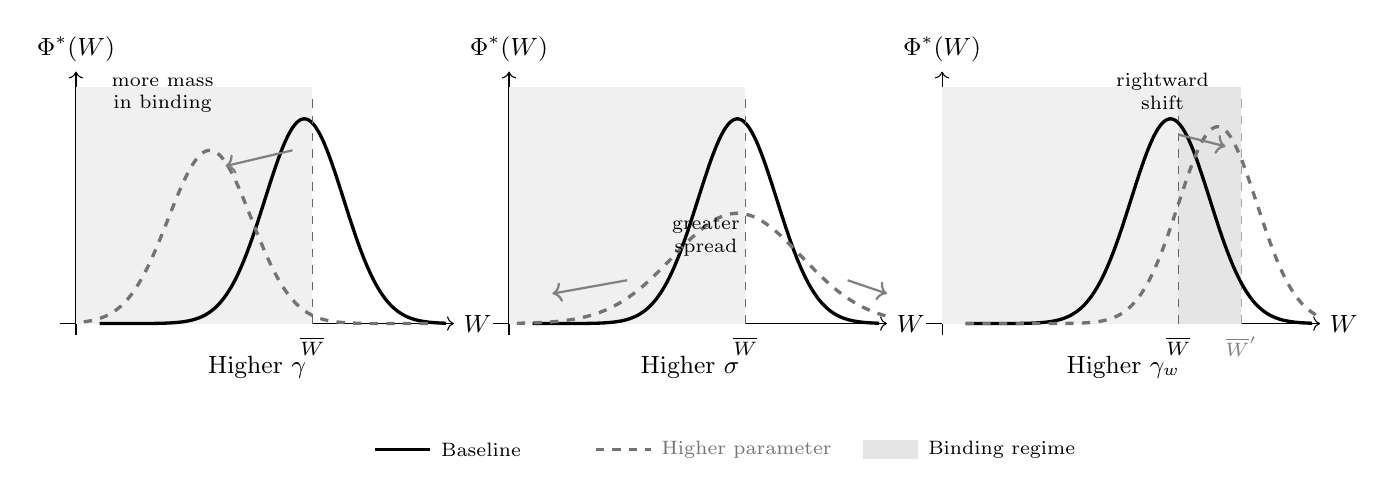
\begin{tikzpicture}[scale=1.0]
 
% Panel 1: effect of gamma
\begin{scope}[xshift=0cm]
    \draw[->] (-0.2,0) -- (4.8,0) node[right, font=\small] {$W$};
    \draw[->] (0,-0.15) -- (0,3.2) node[above, font=\small] {$\Phi^*(W)$};
 
    \fill[gray!12] (0,0) rectangle (3.0,3.0);
 
    \draw[very thick, black, domain=0.3:4.7, smooth, variable=\x, samples=80]
        plot ({\x}, {2.6*exp(-2.0*(\x-2.9)^2)});
 
    \draw[very thick, dashed, black!55, domain=0.1:4.5, smooth, variable=\x, samples=80]
        plot ({\x}, {2.2*exp(-1.8*(\x-1.7)^2)});
 
    \draw[dashed, black!60] (3.0,0) -- (3.0,2.9);
    \node[below, font=\scriptsize] at (3.0,-0.05) {$\overline{W}$};
 
    \draw[->, thick, black!50] (2.75,2.2) -- (1.9,2.0);
 
    \node[font=\small] at (2.3,-0.55) {Higher $\gamma$};
    \node[font=\scriptsize, align=center] at (1.1,2.9) {more mass\\in binding};
\end{scope}
 
% Panel 2: effect of sigma
\begin{scope}[xshift=5.5cm]
    \draw[->] (-0.2,0) -- (4.8,0) node[right, font=\small] {$W$};
    \draw[->] (0,-0.15) -- (0,3.2) node[above, font=\small] {$\Phi^*(W)$};
 
    \fill[gray!12] (0,0) rectangle (3.0,3.0);
 
    \draw[very thick, black, domain=0.3:4.7, smooth, variable=\x, samples=80]
        plot ({\x}, {2.6*exp(-2.0*(\x-2.9)^2)});
 
    \draw[very thick, dashed, black!55, domain=0.1:4.8, smooth, variable=\x, samples=80]
        plot ({\x}, {1.4*exp(-0.75*(\x-2.9)^2)});
 
    \draw[dashed, black!60] (3.0,0) -- (3.0,2.9);
    \node[below, font=\scriptsize] at (3.0,-0.05) {$\overline{W}$};
 
    \draw[->, thick, black!50] (1.5,0.55) -- (0.55,0.38);
    \draw[->, thick, black!50] (4.3,0.55) -- (4.8,0.38);
    \node[font=\scriptsize, align=center] at (2.5,1.1) {greater\\spread};
 
    \node[font=\small] at (2.3,-0.55) {Higher $\sigma$};
\end{scope}
 
% Panel 3: effect of gamma_w
\begin{scope}[xshift=11.0cm]
    \draw[->] (-0.2,0) -- (4.8,0) node[right, font=\small] {$W$};
    \draw[->] (0,-0.15) -- (0,3.2) node[above, font=\small] {$\Phi^*(W)$};
 
    \fill[gray!12] (0,0) rectangle (3.0,3.0);
    \fill[gray!20] (3.0,0) rectangle (3.8,3.0);
 
    \draw[dashed, black!60] (3.0,0) -- (3.0,2.9);
    \node[below, font=\scriptsize] at (3.0,-0.05) {$\overline{W}$};
 
    \draw[dashed, black!35] (3.8,0) -- (3.8,2.9);
    \node[below, font=\scriptsize, text=black!50] at (3.8,-0.05) {$\overline{W}'$};
 
    \draw[very thick, black, domain=0.3:4.7, smooth, variable=\x, samples=80]
        plot ({\x}, {2.6*exp(-2.0*(\x-2.9)^2)});
 
    \draw[very thick, dashed, black!55, domain=0.3:4.8, smooth, variable=\x, samples=80]
        plot ({\x}, {2.5*exp(-2.0*(\x-3.5)^2)});
 
    \draw[->, thick, black!50] (3.0,2.4) -- (3.6,2.25);
    \node[font=\scriptsize, above, align=center] at (2.8,2.6) {rightward\\shift};
 
    \node[font=\small] at (2.3,-0.55) {Higher $\gamma_w$};
\end{scope}
 
% Shared legend
\begin{scope}[xshift=3.8cm, yshift=-1.6cm]
    \draw[very thick, black] (0,0) -- (0.7,0) node[right, font=\scriptsize] {Baseline};
    \draw[very thick, dashed, black!55] (2.8,0) -- (3.5,0) node[right, font=\scriptsize] {Higher parameter};
    \fill[gray!20] (6.2,-0.12) rectangle (6.9,0.12);
    \node[right, font=\scriptsize] at (6.9,0) {Binding regime};
\end{scope}
 
\end{tikzpicture}
\caption*{\text{Source:} Own elaboration.}
\label{fig:ergodic_cs}
\end{figure}
\vspace{-0.2cm}
\begin{remark}[Comparative statics of the exogenous Nash weight $\delta$]\label{rem:delta_cs}
The exogenous bargaining parameter $\delta$ does not affect the two-regime structure of the model but has distinct effects within each regime. We characterize these effects via the Implicit Function Theorem applied to the Nash first-order condition.

\textit{Effect on the equilibrium slope.} In the binding regime, $\beta^*(W)$ satisfies $G(\beta, \underline{w}, \delta) = 0$ where $G := (1-\delta)\Pi'(\beta)/\Pi_s + \delta\,\mathrm{CE}'(\beta)/\mathrm{CE}_s$. Differentiating with respect to $\delta$:
\[
\frac{\partial G}{\partial\delta} = -\frac{\Pi'(\beta^*)}{\Pi_s} + \frac{\mathrm{CE}'(\beta^*)}{\mathrm{CE}_s}.
\]
From the Nash FOC, $\Pi'(\beta^*)/\Pi_s > 0$ and $\mathrm{CE}'(\beta^*)/\mathrm{CE}_s < 0$, so $\partial G/\partial\delta < 0$. Since $\mathrm{SOC} < 0$, where $\mathrm{SOC} := \partial G/\partial\beta\big|_{\beta^*}$ denotes the second-order condition of the Nash problem evaluated at the optimum, the IFT gives
\[
\frac{d\beta^*}{d\delta} = -\frac{\partial G/\partial\delta}{\mathrm{SOC}} = -\frac{(-)}{(-)} < 0.
\]
The calculation above gives $d\beta^*/d\delta < 0$: a higher $\delta$ lowers the equilibrium slope in the binding regime. The economic logic is that a more powerful agent shifts bargaining toward protecting his certainty equivalent rather than bearing additional performance risk, so the equilibrium contract shifts away from incentive pay toward insurance. In the slack regime, by contrast, $\beta^* = \beta^{\mathrm{eff}}$ is independent of $\delta$: when transfers are unconstrained, surplus division and efficiency are separable, and the exogenous bargaining weight affects only $\alpha$, not $\beta$.

\textit{Effect on the regime boundary.} The threshold $\overline{W}$ is defined by the condition that the unconstrained Nash solution exactly satisfies limited liability. The unconstrained solution sets $\alpha^* = \overline{\mathrm{CE}} - C(\beta^{\mathrm{eff}}) + \delta S^{\mathrm{eff}}$, which is strictly increasing in $\delta$. A higher $\delta$ therefore requires a larger fixed payment to satisfy the agent's Nash share, which means the limited liability constraint $\alpha^* \geq \underline{w}(\overline{W}) - \beta^{\mathrm{eff}}\underline{y}$ binds for larger values of $W$. Consequently $\overline{W}$ is strictly increasing in $\delta$: agents with stronger exogenous bargaining power require more accumulated wealth before the unconstrained solution becomes feasible.

\textit{Effect on the ergodic distribution.} The two effects above reinforce each other. A higher $\delta$ raises $\overline{W}$, expanding the binding regime, while simultaneously lowering $\beta^*(W)$ within it, which slows wealth accumulation and makes escaping the binding region harder. Both forces shift the ergodic distribution $\Phi^*$ to the left and increase the long-run mass assigned to $[\underline{W}, \overline{W})$. The bargaining distortion $\Delta(W)$ from Remark \ref{rem:welfare} therefore increases with $\delta$: more powerful agents extract larger shares of surplus through the bargaining protocol rather than through incentive-compatible performance pay, at the cost of greater aggregate efficiency loss in the binding regime.

\textit{Interaction with $\gamma_w$.} When $\gamma_w = 0$ the threshold $\underline{w}$ is exogenous and $\beta^*(W)$ is uniform across the binding domain, so the $\delta$ effect is constant in $W$. When $\gamma_w > 0$, the effect of $\delta$ on $\beta^*(W)$ is heterogeneous: it is largest for low-$W$ agents whose constraints are tightest and whose $\beta^*$ deviates most from $\beta^{\mathrm{eff}}$. The interaction $\partial^2\beta^*/\partial\delta\,\partial W$ is therefore negative under the sign condition of Appendix \ref{ProofProp2}, meaning wealthier agents are less sensitive to changes in $\delta$ within the binding regime.
\end{remark}

The qualitative properties of $\Phi^*$ established here set the terms for the numerical analysis of Section \ref{NumApproach}, which gives quantitative content to each component of Theorem \ref{thm:central} and traces the comparative statics of the ergodic distribution across parameter configurations.

\newpage
%=======================================
\section{Numerical Approach}\label{NumApproach}
%=======================================
 
Theorem \ref{thm:central} establishes three properties of the equilibrium: a two-regime structure in which limited liability determines whether bargaining power is fixed or endogenous, a law of motion for realized bargaining power within the binding regime, and a unique invariant distribution for the wealth process.\footnote{The complete numerical implementation, including all parameter files, value function iteration, simulation routines, and figure scripts, is available at \url{https://github.com/Jean2330/endogenous\_bargaining}.} 

The theoretical analysis characterizes these properties qualitatively but does not yield closed-form expressions for the value and policy functions outside the two limiting cases. This section gives quantitative content to each of the three components. The approach proceeds in three stages: identifying the regime boundary $\overline{W}$ and constructing the wealth grid, iterating the Bellman operators to convergence, and simulating the ergodic distribution and individual wealth paths using the converged policies. This numerical exercise is illustrative rather than a calibration exercise: the parameter values are selected to produce economically interpretable magnitudes and to verify that the qualitative predictions of the theory hold quantitatively rather than to match specific empirical moments.
 
%=======================================
\subsection{Computational algorithms}\label{subsec:algorithms}
%=======================================
 
\subsubsection*{Stage 1: Grid construction and regime identification}
 
The regime boundary $\overline{W}$ is the unique wealth level at which the unconstrained Nash solution exactly satisfies limited liability. It solves
\[
\alpha^{\mathrm{slack}} = \underline{w}(\overline{W}) - \beta^{\mathrm{eff}}\,\underline{y},
\]
where $\alpha^{\mathrm{slack}} := \overline{\text{CE}} - C(\beta^{\mathrm{eff}}) + \delta S^{\mathrm{eff}}$ is the fixed payment the unconstrained Nash solution would set and $\underline{w}(W) = \overline{w} - \gamma_{w}W$ is the wealth-dependent floor. Because $\alpha^{\mathrm{slack}}$ does not depend on $W$ while $\underline{w}$ is strictly decreasing in $W$, the residual is strictly monotone and the root is unique; we locate it by Brent's method.

The upper bound $W_{\max} = \overline{W} + 6\sigma/\!\sqrt{1-\rho^{2}}$ is chosen so that the ergodic distribution assigns negligible mass above $W_{\max}$. At the baseline calibration this gives $W_{\max} \approx 6.7$, which the simulation of Section \ref{subsec:numericalresults} confirms contains essentially all ergodic mass.
 
\begin{algorithm}[H]
\caption{Grid construction and regime identification}
\label{alg:grid}
\begin{algorithmic}[1]
\Require Parameters $(\theta, k, \gamma, \sigma, \rho, \delta,
         \overline{w}, \gamma_{w}, \underline{y},
         \overline{\Pi}, \overline{\text{CE}})$, grid size $N$,
         quadrature order $n_{q}$
\State $\beta^{\mathrm{eff}}
       \leftarrow (\theta^{2}/k)\,/\,(\gamma\sigma^{2}+\theta^{2}/k)$
\State $S^{\mathrm{eff}} \leftarrow S(\beta^{\mathrm{eff}})$,
       \quad $C^{\mathrm{eff}} \leftarrow C(\beta^{\mathrm{eff}})$
\State $\alpha^{\mathrm{slack}}
       \leftarrow \overline{\text{CE}} - C^{\mathrm{eff}} + \delta S^{\mathrm{eff}}$
\State Define $r(W)
       \leftarrow \alpha^{\mathrm{slack}}
       - [\underline{w}(W) - \beta^{\mathrm{eff}}\,\underline{y}]$
\State Solve $r(\overline{W}) = 0$ for $\overline{W}$ via Brent's method
       \Comment{Unique root: $r$ is strictly monotone in $W$}
\State $W_{\min} \leftarrow \epsilon > 0$,\quad
       $W_{\max} \leftarrow \overline{W}
       + 6\sigma/\!\sqrt{1-\rho^{2}}$
\State Construct uniform grid
       $\mathcal{W} \leftarrow \{W_{1}, \ldots, W_{N}\}$
       on $[W_{\min}, W_{\max}]$
\State Compute Gauss-Hermite nodes $\{z_{j}\}$ and weights $\{w_{j}\}$
       of order $n_{q}$
       \Comment{For $\varepsilon \sim \mathcal{N}(0,1)$; see \textcite{judd1998}}
\Ensure Grid $\mathcal{W}$, boundary $\overline{W}$,
        quadrature nodes and weights
\end{algorithmic}
\end{algorithm}
 

 
\subsubsection*{Stage 2: Value function iteration}
 
We iterate the Bellman operators $T_{P}$ and $T_{A}$ defined in equations \eqref{eq:bellman_P}-\eqref{eq:bellman_A} until the sup-norm distance between successive iterates falls below tolerance $\varepsilon_{\mathrm{VFI}}$. Proposition \ref{prop:existence} guarantees convergence from any starting point at geometric rate $\rho$.
 
At each grid point, the solution method depends on the regime induced by the constraint. This regime dependence is central: the constraint not only restricts the feasible set but also alters the nature of surplus sharing, transforming the bargaining problem from transferable utility to non-transferable utility. In the slack regime, the solution is analytic: $\beta^{*} = \beta^{\mathrm{eff}}$ and $\alpha^{*}$ is set to deliver the agent a share $\delta$ of continuation surplus, so $\lambda(W) = \delta$ exactly. In the binding regime, we solve the dynamic Nash first-order condition
\begin{equation}\label{eq:foc_binding_numeric}
G(\beta;\,W,\,V_{P},\,V_{A}) \;:=\;
(1-\delta)\frac{\dfrac{\partial V_P^{b}}{\partial\beta}(W;\beta^*)}{V_P^{b}(W;\beta^*)-\overline{\Pi}}
+
\delta\,\frac{\dfrac{\partial V_A^{b}}{\partial\beta}(W;\beta^*)}{V_A^{b}(W;\beta^*)-\overline{\text{CE}}} \; = \; 0
\end{equation}
for $\beta^{*}(W)$ using Brent's method on the feasible interval. Derivatives $\tfrac{\partial}{\partial\beta} V_P^b$ and $\tfrac{\partial}{\partial\beta} V_A^b$ are computed by central finite differences of order $h = 10^{-5}$ applied to the full quadrature sum, rather than to a spline approximation of the continuation value, to avoid spurious oscillations near the regime boundary. Lemma \ref{lem:beta_bounds} establishes that $G$ changes sign exactly once on the feasible interval, guaranteeing convergence of Brent's method. Expected continuation values $\mathbb{E}[V_{P}(W') \mid W, \beta]$ and $\mathbb{E}[V_{A}(W') \mid W, \beta]$ are evaluated by $n_{q}$-node Gauss-Hermite quadrature, with cubic spline interpolation of the current value function iterates at off-grid wealth levels.
 
\begin{algorithm}[htbp]
\caption{Value function iteration}
\label{alg:vfi}
\begin{algorithmic}[1]
\Require Grid $\mathcal{W}$, boundary $\overline{W}$,
         quadrature $(z_{j}, w_{j})$, parameters,
         tolerance $\varepsilon_{\mathrm{VFI}}$,
         max iterations $T_{\max}$
\State Initialize $V_{P}^{(0)}(W_{i}) \leftarrow 0$,\;
       $V_{A}^{(0)}(W_{i}) \leftarrow 0$ for all $i$
\State $n \leftarrow 0$
\Repeat
    \State Fit cubic splines $\hat{V}_{P}$, $\hat{V}_{A}$
           to $(V_{P}^{(n)}, V_{A}^{(n)})$ on $\mathcal{W}$
    \For{$i = 1$ to $N$}
        \If{$W_{i} \geq \overline{W}$}
            \Comment{Slack regime: analytic solution}
            \State $\beta^{*}(W_{i}) \leftarrow \beta^{\mathrm{eff}}$
            \State $\alpha^{*}(W_{i}) \leftarrow
                   \overline{\text{CE}} - C(\beta^{\mathrm{eff}})
                   + \delta S^{\mathrm{eff}}$
            \State $\lambda(W_{i}) \leftarrow \delta$
        \Else
            \Comment{Binding regime: solve dynamic Nash FOC}
            \State Find feasible interval
                   $[\beta_{\ell}, \beta_{h}] \subset (0,1)$
                   where both $V_{P}^{b}$ and $V_{A}^{b}$ exceed
                   disagreement payoffs
            \State Compute $\tfrac{\partial}{\partial\beta} V_P^b$, $\tfrac{\partial}{\partial\beta} V_A^b$
                   by central finite differences on quadrature sum
            \State Solve $G(\beta;\,W_{i},\,\hat{V}_{P},\,\hat{V}_{A}) = 0$
                   on $[\beta_{\ell}, \beta_{h}]$ via Brent's method
            \State $\alpha^{*}(W_{i})
                   \leftarrow \underline{w}(W_{i})
                   - \beta^{*}(W_{i})\,\underline{y}$
            \State $\lambda(W_{i})
                   \leftarrow (V_{A}^{b} - \overline{\text{CE}})\,/\,
                   [(V_{P}^{b} - \overline{\Pi})
                   + (V_{A}^{b} - \overline{\text{CE}})]$
        \EndIf
        \State Compute $\mathbb{E}[\hat{V}_{P}(W')]$ and
               $\mathbb{E}[\hat{V}_{A}(W')]$ by Gauss-Hermite quadrature
        \State $V_{P}^{(n+1)}(W_{i})
               \leftarrow \Pi(\alpha^{*}, \beta^{*})
               + \rho\,\mathbb{E}[\hat{V}_{P}(W')]$
        \State $V_{A}^{(n+1)}(W_{i})
               \leftarrow \mathrm{CE}(\alpha^{*}, \beta^{*})
               + \rho\,\mathbb{E}[\hat{V}_{A}(W')]$
    \EndFor
    \State $\mathrm{err}^{(n)}
           \leftarrow \max\!\bigl(
           \|V_{P}^{(n+1)} - V_{P}^{(n)}\|_{\infty},\;
           \|V_{A}^{(n+1)} - V_{A}^{(n)}\|_{\infty}\bigr)$
    \State $n \leftarrow n + 1$
\Until{$\mathrm{err}^{(n-1)} < \varepsilon_{\mathrm{VFI}}$
       \textbf{or} $n = T_{\max}$}
\Ensure Converged $V_{P}^{*}$, $V_{A}^{*}$;
        policy functions $\beta^{*}(\cdot)$,
        $\alpha^{*}(\cdot)$, $\lambda(\cdot)$
\end{algorithmic}
\end{algorithm}
 
\subsubsection*{Stage 3: Simulation}
 
Given converged policy functions, we simulate the model forward to characterize the ergodic distribution $\Phi^{*}$ and the dynamics of realized bargaining power along individual paths.
 
\begin{algorithm}[H]
\caption{Simulation of ergodic distribution and bargaining power dynamics}
\label{alg:sim}
\begin{algorithmic}[1]
\Require Converged $\beta^{*}(\cdot)$, $\alpha^{*}(\cdot)$, $\lambda(\cdot)$
         (as cubic splines), boundary $\overline{W}$, parameters,
         $M$ agents, $T$ periods, burn-in $T_{\mathrm{burn}}$
\State Initialize $W_{m}^{(0)} \leftarrow \overline{W}/2$
       for $m = 1, \ldots, M$
       \Comment{Start deep in binding regime}
\For{$t = 1$ to $T$}
    \State Draw $\varepsilon_{m}^{(t)}
           \stackrel{\mathrm{i.i.d.}}{\sim} \mathcal{N}(0,1)$,
           $m = 1, \ldots, M$
    \For{$m = 1$ to $M$}
        \State Evaluate $\beta_{m} \leftarrow \beta^{*}(W_{m}^{(t-1)})$,
               $\alpha_{m} \leftarrow \alpha^{*}(W_{m}^{(t-1)})$,
               $\lambda_{m} \leftarrow \lambda(W_{m}^{(t-1)})$
        \State $a_{m} \leftarrow \beta_{m}\theta/k$,\quad
               $y_{m} \leftarrow \theta a_{m}
               + \sigma\varepsilon_{m}^{(t)}$
        \State $W_{m}^{(t)}
               \leftarrow \mathrm{clip}\!\left(
               \rho_{W} W_{m}^{(t-1)} + \alpha_{m} + \beta_{m}y_{m}
               - \tfrac{k}{2}a_{m}^{2},\;
               W_{\min},\; W_{\max}\right)$
        \State $\ell_{m}^{(t)}
               \leftarrow \log\bigl(\lambda_{m}/(1-\lambda_{m})\bigr)$
    \EndFor
\EndFor
\State Discard periods $1$ through $T_{\mathrm{burn}}$
\State Construct empirical $\hat{\Phi}^{*}$
       from $\{W_{m}^{(t)}\}_{t > T_{\mathrm{burn}}}$
\Ensure Ergodic distribution $\hat{\Phi}^{*}$;
        simulated paths $\{W_{m}^{(t)},\,\lambda_{m}^{(t)},\,
        \ell_{m}^{(t)}\}$
\end{algorithmic}
\end{algorithm}
 
The law of motion in Algorithm \ref{alg:sim} includes a depreciation factor $\rho_W \in (0,1)$, so that $W_{t+1} = \rho_W W_t + \alpha^*(W_t) + \beta^*(W_t) y_t - c(a_t^*)$. This is a computational assumption that does not appear in the theoretical model of Section \ref{Model}, where wealth evolves without depreciation. The role of $\rho_W < 1$ is to ensure that the wealth process is stationary in simulation without requiring a separate mechanism for mean reversion beyond the limited liability channel. At the baseline value $\rho_W = 0.85$, the implied ergodic mean is $W^* \approx 0.95$, which lies just above the regime boundary $\overline{W} = 0.931$, keeping the process active in both regimes. All qualitative conclusions are robust to the choice of $\rho_W$ provided ergodicity is maintained; the quantitative magnitudes reported below correspond to $\rho_W = 0.85$.
 
%=======================================
\subsection{Calibration}\label{subsec:calibration}
%=======================================
 
Table \ref{tab:params} reports the baseline parameter values. The discussion below documents the economic justification for each group and provides literature anchors where available.
 
\begingroup
\small
\setlength{\LTcapwidth}{\textwidth}
\begin{longtable}{lllp{7cm}}
\caption{Baseline parameter values}
\label{tab:params} \\
\toprule
Parameter & Symbol & Value & Interpretation \\
\midrule
\endfirsthead
\multicolumn{4}{l}{\small\textit{Table \ref{tab:params} continued}} \\[2pt]
\toprule
Parameter & Symbol & Value & Interpretation \\
\midrule
\endhead
\midrule
\multicolumn{4}{r}{\small\textit{Continued on next page}} \\
\endfoot
\bottomrule
\endlastfoot
 
\multicolumn{4}{l}{\textit{Technology}} \\[2pt]
Productivity & $\theta$ & $1.0$ &
  Normalization; all output levels are expressed relative to this unit. \\
Effort cost curvature & $k$ & $2.0$ &
  Determines first-best effort $a^{\mathrm{FB}} = \theta/k = 0.50$.
  The ratio $\theta^{2}/k = 0.50$ governs the slope of the incentive-effort trade-off. \\[6pt]
 
\multicolumn{4}{l}{\textit{Preferences}} \\[2pt]
Risk aversion & $\gamma$ & $1.0$ &
  CARA coefficient. Combined with $\sigma$, gives risk premium $\gamma\sigma^{2}/2 = 0.045$,
  within the range in the dynamic contracting literature \parencite{holmstrom1987, haubrich1994}. \\
Discount factor & $\rho$ & $0.95$ &
  Annual discount rate of approximately 5 percent, the standard
  value in dynamic macro and contracting models \parencite{stokey1989}. \\[6pt]
 
\multicolumn{4}{l}{\textit{Output}} \\[2pt]
Volatility & $\sigma$ & $0.3$ &
  Output standard deviation. At baseline, $\beta^{\mathrm{eff}} \approx 0.847$ and
  $S^{\mathrm{eff}} \approx 0.212$. Comparative statics vary $\sigma \in \{0.15, 0.30, 0.45, 0.60\}$. \\
Output lower bound & $\underline{y}$ & $-0.5$ &
  The parameter entering the limited liability constraint $\alpha \geq \underline{w}(W) - \beta\underline{y}$.
  Since output follows $y = \theta a + \sigma\varepsilon$ with $\varepsilon \sim \mathcal{N}(0,1)$,
  realized output can be negative in the left tail.
  Setting $\underline{y} < 0$ ensures the constraint has empirical content:
  a value of zero would make the binding region negligibly small under the normal distribution.
  With mean output $\mu_y \approx 0.42$ at baseline effort,
  $\underline{y} = -0.5$ lies approximately 3.1 standard deviations below the mean. \\[6pt]

\pagebreak[4]
\multicolumn{4}{l}{\textit{Bargaining}} \\[2pt]
Nash weight & $\delta$ & $0.4$ &
  Exogenous bargaining weight on the agent. A value below $0.5$ gives the principal
  structural advantage, consistent with employment relationships \parencite{binmore1986}.
  Comparative statics of $\delta$ are characterized in Remark \ref{rem:delta_cs}. \\[6pt]
 
\multicolumn{4}{l}{\textit{Limited liability}} \\[2pt]
LL floor intercept & $\overline{w}$ & $-0.30$ &
  Intercept of $\underline{w}(W) = \overline{w} - \gamma_{w}W$. Calibrated jointly
  with $\gamma_w$ so that the regime boundary falls at $\overline{W} \approx 0.931$,
  an interior point of the wealth grid visible in all figures. \\
Wealth elasticity & $\gamma_{w}$ & $0.20$ &
  Rate at which the LL floor relaxes with wealth. A value below 1 satisfies the
  ergodicity condition of Proposition \ref{prop:ergodic}. The mechanism shuts
  down at $\gamma_{w} = 0$, which serves as the benchmark.
  Comparative statics vary $\gamma_w \in \{0.05, 0.10, 0.20, 0.35\}$. \\[6pt]
 
\multicolumn{4}{l}{\textit{Outside options}} \\[2pt]
Disagreement payoffs & $\overline{\Pi}, \overline{\text{CE}}$ & $0$ &
  Both disagreement payoffs are set to zero. This ensures that realized
  bargaining power in the slack regime equals the exogenous Nash weight exactly,
  $\lambda = \delta$, providing a clean baseline against which to measure
  the binding-regime deviation. \\[6pt]

\pagebreak[4]
\multicolumn{4}{l}{\textit{Computational settings}} \\[2pt]
Wealth depreciation & $\rho_W$ & $0.85$ &
  Depreciation factor in the simulation law of motion $W_{t+1} = \rho_W W_t + \ldots$.
  This is a computational assumption not present in the theoretical model; it
  ensures stationarity of simulated paths. At this value the ergodic mean
  satisfies $W^* \approx 0.95 > \overline{W}$. \\
Grid points & $N$ & $300$ &
  Uniform grid on $[0.05, W_{\max}]$. Increasing to $N = 500$ leaves all
  reported statistics unchanged to two decimal places. \\
Quadrature nodes & $n_{q}$ & $10$ &
  Gauss-Hermite nodes for $\varepsilon \sim \mathcal{N}(0,1)$.
  Ten nodes are exact for polynomials of degree up to 19 \parencite{judd1998}. \\
VFI tolerance & $\varepsilon_{\mathrm{VFI}}$ & $10^{-6}$ &
  Sup-norm convergence criterion. \\
Simulation & $M \times T$ & $1000 \times 10000$ &
  1{,}000 agents each simulated for 10{,}000 periods with $T_{\mathrm{burn}} = 500$,
  yielding 9.5 million agent-period observations for the ergodic distribution. \\
 
\end{longtable}
\endgroup
 
Table \ref{tab:derived} reports the derived model statistics implied by the baseline calibration.
 
\begin{table}[htbp]
\centering
\caption{Derived model statistics at the baseline calibration}
\label{tab:derived}
\begin{tabular}{lll}
\toprule
Statistic & Symbol & Value \\
\midrule
Efficient incentive slope & $\beta^{\mathrm{eff}}$ & $0.847$ \\
First-best effort & $a^{\mathrm{FB}}$ & $0.500$ \\
Efficient effort & $a^{\mathrm{eff}}$ & $0.424$ \\
First-best surplus & $S^{\mathrm{FB}}$ & $0.250$ \\
Efficient surplus & $S^{\mathrm{eff}}$ & $0.212$ \\
Moral hazard efficiency loss & $S^{\mathrm{FB}} - S^{\mathrm{eff}}$ & $0.038$ \\
Agent disagreement payoff & $\overline{\text{CE}}$ & $0$ \\
Principal disagreement payoff & $\overline{\Pi}$ & $0$ \\
Regime boundary & $\overline{W}$ & $0.931$ \\
Wealth grid & $[W_{\min}, W_{\max}]$ & $[0.05,\;6.70]$ \\
VFI convergence & Iterations & $\approx 229$ \\
Ergodic mean wealth & $\mathbb{E}_{\Phi^*}[W]$ & $0.784$ \\
Prob.\ in binding regime & $\Pr(W_t < \overline{W})$ & $0.659$ \\
Ergodic mean $\lambda$ & $\mathbb{E}_{\Phi^*}[\lambda]$ & $0.411$ \\
Mean $\lambda$ conditional on binding & $\mathbb{E}[\lambda \mid W < \overline{W}]$ & $0.417$ \\
\bottomrule
\end{tabular}
\end{table}
 
Two features of the calibration deserve specific comment. First, setting both disagreement payoffs to zero ($\overline{\Pi} = \overline{\text{CE}} = 0$) is not an approximation but a deliberate identification choice. It ensures that the slack-regime identity $\lambda = \delta$ holds exactly rather than approximately, which provides the sharpest possible baseline for measuring the binding-regime deviation. Any positive disagreement payoff would shift both value functions uniformly, leaving the deviation $\lambda(W) - \delta$ unchanged in sign and direction, but would introduce a constant that partially obscures the comparison. Second, the parameters $\overline{w}$ and $\gamma_w$ do not have direct empirical counterparts in the existing literature, since wealth-dependent limited liability is the novel ingredient of the model. They are chosen to satisfy two requirements: the feasible set is non-empty across the entire binding domain, and the regime boundary lies at an interior point of the wealth grid where the mechanism is active in the ergodic distribution. Any calibration satisfying $\gamma_w \in (0,1)$ and $\overline{W}$ interior preserves all qualitative results.
 
%=======================================
\subsection{Numerical results}\label{subsec:numericalresults}
%=======================================
 
We organize the results around the three theoretical claims of Section \ref{Model}: that the equilibrium slope and realized bargaining power are both monotone functions of wealth in the binding regime; that they converge to their slack-regime values at the boundary $\overline{W}$; and that the wealth process admits a unique ergodic distribution with properties governed by the parameters $\gamma$, $\sigma$, and $\gamma_w$.

 
Figure \ref{fig:policy_functions} displays the three principal policy functions over the wealth grid. In the binding regime ($W < \overline{W} = 0.931$), the equilibrium slope $\beta^*(W)$ lies strictly below the efficient benchmark $\beta^{\mathrm{eff}} = 0.847$, rising monotonically from approximately $0.667$ at the lower end of the grid to $\beta^{\mathrm{eff}}$ at $\overline{W}$. This confirms Proposition \ref{prop:tu_ntu}: when limited liability binds, the Nash solution requires $\beta^*(W) < \beta^{\mathrm{eff}}$ and the distortion closes as wealth relaxes the constraint. Above $\overline{W}$ the slope is constant at $\beta^{\mathrm{eff}}$, consistent with the slack regime in which $\alpha^*$ adjusts freely.
 
The center panel of Figure \ref{fig:policy_functions} shows realized bargaining power $\lambda(W)$. In the binding regime, $\lambda(W) > \delta = 0.40$ throughout, with the deviation reaching approximately $0.437$ at the lower end of the grid. The direction of the inequality follows from the sufficient condition \eqref{eq:lambda_sign_condition} of Appendix \ref{ProofProp2}, which is satisfied at the baseline calibration: the agent captures more than the exogenous Nash share when limited liability binds. The function is monotone decreasing in $W$ on the binding domain, converging to $\delta$ at $\overline{W}$. In the slack regime $\lambda(W) = \delta = 0.40$ exactly at every grid point, as the theory predicts. This is the central numerical verification of the paper: the wedge $\lambda(W) - \delta$ is positive, monotone in $W$, and vanishes precisely at the regime boundary.
 
The right panel shows the welfare distortion $\Delta(W) = S^{\mathrm{eff}} - S(\beta^*(W))$. This is zero throughout the slack regime and rises as $W$ falls below $\overline{W}$, reaching approximately $0.010$ at the lower end of the grid. The pattern confirms the welfare decomposition of Remark \ref{rem:welfare}: the cost of the endogenous bargaining mechanism is concentrated among agents with low accumulated wealth and is negligible near the regime boundary.
 
\begin{figure}[H]
\centering
\caption{Policy functions at baseline. Left: $\beta^*(W)$ below $\beta^{\mathrm{eff}}$ in the binding regime. Center: $\lambda(W) > \delta$ in the binding regime, equal to $\delta$ in the slack. Right: welfare distortion $\Delta(W)$. Dotted line at $\overline{W} = 0.931$.}

\includegraphics[width=\textwidth]{Figuras/fig_policy_functions.png}
\caption*{\text{Source:} Own elaboration in Python.}
\label{fig:policy_functions}
\end{figure}
 
Figure \ref{fig:value_functions} shows the value functions $V_P(W)$ and $V_A(W)$. Both exhibit the kink at $\overline{W}$ established in Remark \ref{rem:boundary}: the slope changes discontinuously at the regime boundary, though the level is continuous. The principal's value $V_P(W)$ is increasing and concave on the binding domain, then flattens above $\overline{W}$ as further wealth accumulation does not relax the limited liability constraint. The agent's value $V_A(W)$ is increasing throughout: higher wealth relaxes the constraint, reducing the distortion in $\beta^*$ and raising total surplus. Both value functions are consistent with the contraction mapping result of Proposition \ref{prop:existence}.
 
\begin{figure}[H]
\centering
\caption{Value functions $V_P(W)$ and $V_A(W)$. Both are continuous at $\overline{W} = 0.931$ (dotted line) with a slope change at the regime boundary.}

\includegraphics[width=0.75\textwidth]{Figuras/fig_value_functions.png}
\caption*{\text{Source:} Own elaboration in Python.}
\label{fig:value_functions}
\end{figure}
\vspace{-0.1cm}

Figure \ref{fig:pareto_frontiers} provides the geometric intuition for the two-regime structure by displaying the Pareto frontier in $(\Pi_s, \mathrm{CE}_s)$ space for both regimes alongside the Nash solution in each. In the slack regime the frontier is linear, and the Nash solution (the point where an iso-Nash curve is tangent to the frontier) delivers the agent exactly the share $\delta$ of total surplus. In the binding regime the frontier is curved, and the Nash solution delivers a share $\lambda^{\mathrm{bind}} \neq \delta$ because redistributing surplus requires moving along the curved frontier rather than adjusting the fixed payment.

Figure \ref{fig:ergodic} displays the simulated ergodic distribution $\hat{\Phi}^*$ constructed from 1{,}000 agents each simulated for 10{,}000 periods with a burn-in of 500. The distribution is unimodal and right-skewed, with its mode slightly below $\overline{W} = 0.931$ (marked by the dashed vertical line). Approximately 65.9 percent of the ergodic mass falls in the binding regime ($W < \overline{W}$), indicating that the endogenous bargaining mechanism is active for a majority of the stationary population at any given date. The right tail extends to $W \approx 3$, reflecting agents who have accumulated substantially and operate in the slack regime. The distribution is consistent with the Foster-Lyapunov condition of Proposition \ref{prop:ergodic}: the drift coefficient $-2\gamma_w(1-\gamma_w) = -0.32 < 0$ at $\gamma_w = 0.20$ ensures mean reversion, producing the concentrated stationary shape visible in the figure.
 
\begin{figure}[H]
\centering
\caption{Pareto frontiers. Left: slack regime, linear frontier, $\lambda = \delta$. Right: binding regime at $W = \overline{W}/2$, curved frontier, $\lambda \neq \delta$. Dashed curves are iso-Nash-product loci $\Pi_s^{1-\delta}\,\mathrm{CE}_s^{\delta} = \text{const}$ at $\delta = 0.4$; they are not egalitarian ($\delta \neq 0.5$) but are tangent to the frontier at the respective Nash solutions.}

\includegraphics[width=0.7\textwidth]{Figuras/fig_pareto_frontiers.png}
\caption*{Source: Own elaboration in Python.}
\label{fig:pareto_frontiers}
\end{figure}
\vspace{-0.1cm}
 
\begin{figure}[H]
\centering
\caption{Simulated ergodic distribution $\hat{\Phi}^*$. Dashed line at $\overline{W} = 0.931$; shaded region is the binding regime (65.9\% of mass). Ergodic mean $W^* \approx 0.784$.}

\includegraphics[width=0.70\textwidth]{Figuras/fig_ergodic.png}
\caption*{Source: Own elaboration in Python.}
\label{fig:ergodic}
\end{figure}
\vspace{-0.1cm}
 
Figure \ref{fig:single_path} shows a representative simulated path of $W_t$ and $\lambda_t$ over 200 periods. The upper panel shows $W_t$ fluctuating around $\overline{W}$, crossing the boundary in both directions. The lower panel shows the corresponding realized bargaining power: when $W_t < \overline{W}$, $\lambda_t$ lies above $\delta = 0.40$, reaching values near $0.437$ in binding episodes; when $W_t \geq \overline{W}$, $\lambda_t$ drops to $\delta$ exactly. The switching between regimes is immediate and state-dependent. This is the correct interpretation of Proposition \ref{prop:dynamics}: $\lambda_t$ evolves because $W_t$ evolves through the policy function $\lambda(\cdot)$, not because $\lambda$ itself is a separate state variable with its own law of motion. The figure also illustrates the distribution of realized bargaining power in log-odds space $\ell_t = \log(\lambda_t / (1-\lambda_t))$, which fluctuates between the binding-regime value $\ell^{\mathrm{bind}} \approx 0.30$ and the slack-regime constant $\ell^{\mathrm{slack}} = \log(\delta/(1-\delta)) \approx -0.405$.
 
\begin{figure}[H]
\centering
\caption{Simulated path of $W_t$ (upper) and $\lambda_t$ (lower). Dashed lines at $\overline{W} = 0.931$ and $\delta = 0.40$. Episodes with $W_t < \overline{W}$ coincide with $\lambda_t > \delta$.}

\includegraphics[width=\textwidth]{Figuras/fig_single_path.png}
\caption*{Source: Own elaboration in python.}
\label{fig:single_path}
\end{figure}
  
Figures \ref{fig:cs_gamma}, \ref{fig:cs_sigma}, and \ref{fig:cs_gamma_w} display the comparative statics of the ergodic distribution with respect to $\gamma$, $\sigma$, and $\gamma_w$ respectively. Each figure holds the remaining parameters at their baseline values and varies the focal parameter across four levels. Dotted vertical lines mark $\overline{W}$ for each parameterization.
 
As risk aversion $\gamma$ rises, the ergodic distribution shifts leftward and concentrates more mass in the binding regime. Higher risk aversion reduces $\beta^{\mathrm{eff}}$ through the Holmstrom-Milgrom mechanism, which lowers expected income and makes it harder for agents to accumulate above $\overline{W}$. The threshold $\overline{W}$ itself shifts rightward with $\gamma$, since the unconstrained Nash solution that defines the boundary uses $\beta^{\mathrm{eff}}$ and a more risk-averse agent requires a larger fixed payment to achieve the $\delta$ Nash share. The interaction of a leftward-shifting distribution with a rightward-shifting threshold implies that the fraction of time spent in the binding regime rises sharply with $\gamma$.
 
\begin{figure}[H]
\centering
\caption{Ergodic distribution $\hat{\Phi}^*$ for $\gamma \in \{0.5, 1.0, 1.5, 2.0\}$. Higher $\gamma$ shifts mass leftward and moves $\overline{W}$ (dotted lines) rightward.}

\includegraphics[width=0.8\textwidth]{Figuras/fig_cs_gamma.png}
\caption*{Source: Own elaboration in Python.}
\label{fig:cs_gamma}
\end{figure}
\vspace{-0.1cm}
 
As output volatility $\sigma$ rises, the ergodic distribution spreads and its mean falls. Higher volatility reduces $\beta^{\mathrm{eff}}$, which lowers average wealth accumulation, while also directly increasing the variance of wealth innovations $\beta^*(W)\sigma\varepsilon_t$. The threshold $\overline{W}$ falls with $\sigma$ because the unconstrained fixed payment decreases as $\beta^{\mathrm{eff}}$ falls. The net effect is a broader, lower-mean distribution at high volatility, with more mass on both sides of the (lower) threshold.
 
\begin{figure}[H]
\centering
\caption{Ergodic distribution $\hat{\Phi}^*$ for $\sigma \in \{0.15, 0.30, 0.45, 0.60\}$. Higher $\sigma$ spreads the distribution and moves $\overline{W}$ (dotted lines) leftward.}

\includegraphics[width=0.8\textwidth]{Figuras/fig_cs_sigma.png}
\caption*{Source: Own elaboration in Python.}
\label{fig:cs_sigma}
\end{figure}
\vspace{-0.1cm}
 
As the wealth elasticity $\gamma_w$ rises, the ergodic distribution shifts rightward and its right tail lengthens. A higher $\gamma_w$ means the limited liability floor relaxes more slowly with wealth, so agents must accumulate more to exit the binding regime. The threshold $\overline{W}$ rises with $\gamma_w$. Higher $\gamma_w$ also amplifies the sensitivity $\lambda'(W)$ through its direct appearance in the derivative of the limited liability floor (Appendix \ref{ProofProp2}), so agents in the binding regime experience larger period-to-period movements in realized bargaining power for the same output shock. This is the clearest quantitative illustration of the paper's main mechanism: the parameter governing how wealth relaxes the limited liability constraint directly controls both the location of the ergodic distribution and the amplitude of bargaining power fluctuations within the binding regime.
 
\begin{figure}[H]
\centering
\caption{Ergodic distribution $\hat{\Phi}^*$ for $\gamma_w \in \{0.05, 0.10, 0.20, 0.35\}$. Higher $\gamma_w$ shifts the distribution rightward and moves $\overline{W}$ (dotted lines) rightward.}

\includegraphics[width=0.85\textwidth]{Figuras/fig_cs_gamma_w.png}
\caption*{Source: Own elaboration in Python.}
\label{fig:cs_gamma_w}
\end{figure}
  
Figure \ref{fig:comparison_ss} provides a direct numerical comparison with \textcite{spear1987}. We implement their model with the same output distribution, effort set, and discount factor used here, applying CARA utility to maintain comparability with the contract space. Three contrasts emerge. First, the value functions occupy different state spaces: the SS value function $V(v_t)$ is defined over promised utility, while $V_P(W)$ is defined over wealth. Both are concave, but the kink in $V_P(W)$ at $\overline{W}$ has no analogue in the SS formulation, reflecting the regime-switching structure absent in their model. Second, the incentive slope in SS equals $\beta^{\mathrm{eff}}$ everywhere by the standard Holmstrom-Milgrom result; in this model $\beta^*(W) < \beta^{\mathrm{eff}}$ in the binding regime, with the gap reflecting the bargaining distortion $\Delta(W)$. Third, wage sensitivity to output shocks, measured by $w_H(v_t) - w_L(v_t)$ in SS and by $\beta^*(W)\sigma$ in this model, shows a similar level across the two models in the slack region but a reduction in the binding regime, as the lower $\beta^*$ implies less exposure to output risk.
 
\begin{figure}[H]
\centering
\caption{Comparison with \textcite{spear1987}. Left two panels: $V(v_t)$ (blue) and $V_P(W)$ (red) in their respective state spaces. Third: $\beta^*(W)$ below the SS benchmark $\beta^{\mathrm{eff}}$ in the binding regime. Fourth: wage sensitivity to output shocks, normalized by state variable range.}

\includegraphics[width=\textwidth]{Figuras/fig_comparison_ss.png}
\caption*{Source: Own elaboration in Python.}
\label{fig:comparison_ss}
\end{figure}
 
Figure \ref{fig:comparison_dg} provides the analogous comparison with \textcite{digiannatale2025}. Three panels are shown. The first compares the mean conditional drift of the bargaining state across models. In the DG framework, the expected change in bargaining power is constant and positive in every period, equal to the bargaining drift coefficient $(f_{HH} - f_{LH} [ y_L/y_H])\varepsilon \approx 0.0005$ at the baseline. In this model, the analogous quantity $\mathbb{E}[\lambda(W_{t+1}) \mid W_t] - \lambda(W_t)$ is computed by quadrature from the converged policy functions and is strongly state-dependent: it is positive for $W_t < W^*$, crosses zero at the ergodic mean $W^* \approx 0.784$, and is negative for $W_t > W^*$. The region labels in the figure identify where the limited liability constraint is binding and where it is slack. This mean-reversion property cannot be generated by any constant-drift specification. The second panel compares performance pay intensity, normalized by the respective output range to isolate incentive intensity from levels: the DG wage differential $w_H(\delta) - w_L(\delta)$ divided by $y_H - y_L$ is nearly constant across the state, while the corresponding quantity $\beta^*(W)(E[y_H \mid W] - \underline{y})/\overline{(y_H - y_L)}$ rises with $W$ in the binding regime and flattens in the slack regime. The third panel shows simulated paths of the bargaining state from three initial conditions in each model: DG paths drift slowly and nearly deterministically upward, while paths in this model fluctuate rapidly around the ergodic mean, crossing the Nash weight $\delta = 0.40$ repeatedly in both directions.
 
\begin{figure}[H]
\centering
\caption{Comparison with \textcite{digiannatale2025}. Left: mean drift of the bargaining state, constant in DG and mean-reverting in this model. Center: performance pay intensity normalized by output range. Right: simulated paths from three initial conditions; dashed line at $\delta = 0.40$.}

\includegraphics[width=\textwidth]{Figuras/fig_comparison_dg.png}
\caption*{Source: Own elaboration in Python.}
\label{fig:comparison_dg}
\end{figure}

The convergence of the value function iteration documented in Table \ref{tab:derived} provides numerical verification that the equilibrium mapping is well-behaved in the long run. In the spirit of \textcite{abreu1990}, one can think of the set of continuation value pairs $(V_P(W), V_A(W))$ as needing to be self-generating under the induced policy functions: the equilibrium continuation values at any state $W$ must be reproducible by the stationary contract $(\alpha^*(W), \beta^*(W))$ together with the continuation values that follow from next period's wealth.  The convergence of value functions to a fixed point is confirmed by numerical results. In about 229 iterations they approach unique pair $(V_P^*, V_A^*)$ that will be stable under the bellman operator applications. Similarly, the ergodic distribution $\hat{\Phi}^*$, which was obtained from simulation data, has this same property of stability. The wealth process initialized at any point on interval $ [W_{\min}, W_{\max}] $ will tend to the same equilibrium distribution as it evolves over time and does not depend on the initial condition of the system; this is consistent with geometric ergodicity proven in proposition \ref{prop:ergodic}.

Ergodic mass distribution simulated $\hat{\Phi}^*$ provides a physical interpretation for long-run heterogeneity established in proposition \ref{prop:ergodic}. Agents with identical primitive characteristics but different output history will have different positions on schedule $\lambda(W)$ forever. Those whose output history place them below $\overline{W}$ have curved frontier and realize surplus share that deviates from $\delta$, while those above $\overline{W}$ work as if in standard transferable utility framework. Mass of 65.9\% of ergodic mass fell into binding regime is not just a transient phenomena, it reflects steady state of wealth process under baseline calibration and is therefore perpetually present in parameterization where $\gamma_w \in (0,1)$, structural drift $\kappa_t = \gamma_w \beta_t^* \sigma$ governing the distribution is observable in principle and can be derived from panel data on long-term compensation contracts. This suggests a natural empirical extension in which the structural parameters are recovered from data on contract terms, firm performance, and measures of the agent's financial position, using the identification approach of \textcite{digiannatale2025} as a starting point.

\newpage
 
%=======================================
\section{Conclusion}\label{Conclusion}
%=======================================
This thesis demonstrates that limited liability is capable of creating bargaining 
power, instead of simply limiting bargains. With the level of limited liability determined 
by the amount of wealth an individual has amassed, the Pareto frontier is no longer a 
straight line (as it would be without limited liability), and the only possible tool to 
use to redistribute surplus is the incentive slope, $\beta_t$. Therefore, as the value 
of $\beta_t$ increases or decreases, both the total amount of surplus created and the 
allocation of that surplus among agents will increase or decrease. Thus, while the value 
of $\beta_t$ can be used to make the distribution of surplus more equitable, it also 
creates an inefficiency. That is, it is impossible to create equity in the allocation of 
surplus without creating some degree of inefficiency.

Given that it is not possible to separate issues of equity and efficiency when using the 
incentive slope, the Nash bargaining solution over the non-transferable utility frontier 
will result in a realized share $\lambda(W)$ that differs from the exogenous Nash weight 
$\delta$. Importantly, the difference between $\lambda(W)$ and $\delta$ will depend upon 
an agent's wealth at date $t$, $W_t$, and thus will be history dependent. Furthermore, 
the dependence of bargaining power on wealth implies that bargaining power is not 
something that evolves over time due to external events (such as a change in an agent's 
patience, outside option, or Nash weight). Rather, bargaining power is an endogenous 
state variable generated by the interplay between an agent's wealth accumulation and the 
binding limited liability constraint.

It is the existence of a unique invariant distribution $\Phi^*$ that eliminates the 
possibility that this mechanism can be dismissed as a transitionary phenomenon. The 
wealth process generates a stochastic steady-state distribution $\Phi^*$ such that there 
is persistent mass within the binding regime. Specifically, in my base case calibration, 
65.9\% of the ergodic distribution lies within the binding regime. Furthermore, agents 
with identical primitives (i.e., same patience, same outside option, etc.) who experience 
different histories of outputs will find themselves located permanently in different 
locations along the $\lambda(W)$ schedule. The source of this permanent heterogeneity is 
the cumulative impact of previous output shocks on each agent's current wealth. It is 
this wealth that determines each agent's location relative to the limited liability 
threshold.

Classical dynamic contracting literature \parencite{holmstrom1979, spear1987, thomas1990} 
treats bargaining power as an exogenous input to the contracting problem, examining how 
incentives and continuation values evolve within that framework. Traditional Nash bargaining literature \parencite{nash1950, rubinstein1982, binmore1986} examines surplus 
division given a fixed and feasible set of allocations. \textcite{demougin2006} 
demonstrate that in a static environment with limited liability and risk-neutral parties, 
there exist three equivalent representations of bargaining power on the Pareto frontier. 
Importantly, none of these works examines whether binding limited-liability constraints 
can transform bargaining power from an exogenous primitive into an endogenous state 
variable. \textcite{digiannatale2025} examine how the drift in bargaining power evolves 
over time in a reduced-form setting. This thesis develops structural microfoundations 
that provide the basis for understanding why and how bargaining power drifts over time 
due to binding limited-liability constraints.

The structural drift $\kappa_t = \gamma_w \beta_t^* \sigma$ is potentially identifiable 
from data. It depends solely upon the incentive slope $\beta_t^*$, output volatility 
$\sigma$, and the wealth elasticity of the limited liability floor $\gamma_w$, each 
having direct analogues in panel data on long-term compensation contracts. Given the 
identification method developed by \textcite{digiannatale2025}, their reduced-form 
estimate $\hat{\kappa}$ maps directly into this structural representation. Controlling 
for both $\beta_t^*$ and $\sigma$ would allow $\gamma_w$ to be isolated as the residual. 
From a policy perspective, the fact that $\Delta(W)$ is decreasing in wealth and 
disappears once $\overline{W}$ is reached provides one reason to consider instruments 
designed to shift the ergodic distribution to the right. The theorem establishes that a 
welfare distortion does exist and describes its size; however, whether any particular 
intervention is desirable depends on factors outside the scope of this study.

More generally, this thesis demonstrates that observed changes in bargaining outcomes  need not be indicative of underlying changes in bargaining fundamentals. In the model,  an agent may receive a greater share of surplus over time despite experiencing no change  in patience, outside options, or exogenous Nash weights. The only reason for this change  is that accumulated wealth reduces the binding limited liability constraint, thereby  expanding the feasible set of allocations and shifting the agent's bargaining position  along the Pareto frontier. The key lesson is that bargaining power need not be treated  as primitive. Under wealth-dependent limited liability, it emerges endogenously as part of the contractual environment itself.
\newpage
\addcontentsline{toc}{section}{References}
\printbibliography

\newpage
\begin{appendices}
    %==========================================
    \section{Appendix A: Connection to Reduced-Form Dynamics} \label{ReducedFormDynamics}
    %==========================================

    The structural model in Section \ref{Model} derives bargaining power evolution from the interaction of binding limited liability constraints and wealth accumulation. This appendix shows how the mechanism maps to the reduced-form stochastic processes used in computational approaches \parencite{digiannatale2025}.
    
    In a dynamic setting, the disagreement payoffs $(\overline{\Pi}_t, \overline{\text{CE}}_t)$ represent the principal's profit and the agent's certainty equivalent if negotiations break down at date $t$. In the theoretical model of Section \ref{Model} these are treated as fixed exogenous constants $(\overline{\Pi}, \overline{\text{CE}})$. This appendix considers an extension for the purpose of the mapping exercise only: suppose that disagreement payoffs depend on expected future interactions and are therefore influenced by current performance. To trace the structural implications of that channel, we posit linear updating rules
    \[
    \overline{\Pi}_{t+1} = \overline{\Pi}_t + [(y_t - w_t) - \mathbb{E}[y_t - w_t \mid a_t^*]]\xi_P ,
    \]
    \[
    \overline{\text{CE}}_{t+1} = \overline{\text{CE}}_t + [w_t - \mathbb{E}[w_t \mid a_t^*]]\xi_A ,
    \]
    where $\xi_P, \xi_A > 0$ capture how realized deviations from expected payoffs propagate into future disagreement payoffs. This updating structure is not a maintained assumption of the model; it is a device for connecting the structural sensitivity $\gamma_w$ to the reduced-form drift $\kappa$ of \textcite{digiannatale2025}.
    
    Under the linear contract $w_t = \alpha_t + \beta_t y_t$ with $y_t = \theta a_t^* + \sigma \varepsilon_t$, realized deviations from expectations are
    \[
    w_t - \mathbb{E}[w_t \mid a_t^*] = \beta_t \sigma \varepsilon_t, \qquad (y_t - w_t) - \mathbb{E}[y_t - w_t \mid a_t^*] = (1-\beta_t) \sigma \varepsilon_t.
    \]
    Substituting these into the threat-point evolution equations yields
    \[
    \overline{\Pi}_{t+1} = \overline{\Pi}_t + \xi_P (1-\beta_t) \sigma \varepsilon_t, \qquad \overline{\text{CE}}_{t+1} = \overline{\text{CE}}_t + \xi_A \beta_t \sigma \varepsilon_t.
    \]
    
    Changes in threat points induce changes in realized bargaining power through the Nash first-order condition. When limited liability binds, the equilibrium slope $\beta_t^*$ satisfies
    \[
    (1-\delta) \frac{\Pi_t'(\beta_t^*)}{\Pi_t(\beta_t^*) - \overline{\Pi}_t} + \delta \frac{\text{CE}_t'(\beta_t^*)}{\text{CE}_t(\beta_t^*) - \overline{\text{CE}}_t} = 0.
    \]
    The implicit function theorem gives
    \[
    \frac{\partial \beta_t^*}{\partial \overline{\Pi}_t} = -\frac{(1-\delta)[\Pi_t'(\beta_t^*)]^2}{[\Pi_t(\beta_t^*) - \overline{\Pi}_t]^2\ \text{SOC}}, \qquad \frac{\partial \beta_t^*}{\partial \overline{\text{CE}}_t} = -\frac{\delta[\text{CE}_t'(\beta_t^*)]^2}{[\text{CE}_t(\beta_t^*) - \overline{\text{CE}}_t]^2 \text{SOC}}
    \]
    where $\text{SOC} < 0$ is the second-order condition. Denote the sensitivities of realized bargaining power to threat points by
    \[
    \frac{\partial \lambda_t}{\partial \overline{\Pi}_t} = -\mu_P, \qquad \frac{\partial \lambda_t}{\partial \overline{\text{CE}}_t} = \mu_A.
    \]
    
    For small changes, the evolution of realized bargaining power can be approximated as
    \[
    \lambda_{t+1} - \lambda_t \approx [-\mu_P \xi_P (1-\beta_t) + \mu_A \xi_A \beta_t] \sigma \varepsilon_t.
    \]
    Define the composite sensitivity
    \[
    \tilde{\kappa}_t := [-\mu_P \xi_P (1-\beta_t) + \mu_A \xi_A \beta_t] \sigma.
    \]
    
    Working in log-odds space, the chain rule gives
    \[
    \ell_{t+1} - \ell_t \approx \frac{\tilde{\kappa}_t \varepsilon_t}{\lambda_t(1-\lambda_t)}.
    \]
    Mean reversion arises from discounting and the boundedness of feasible allocations. In the reduced form, this is captured by a persistence parameter $\phi \in (0,1)$, giving
    \[
    \ell_{t+1} = (1-\phi)\overline{\ell} + \phi \ell_t + \tilde{\kappa}_t \varepsilon_t.
    \]
    
    The structural and reduced-form approaches are connected through parameter mappings. When the principal's channel dominates, the composite drift simplifies to $\tilde{\kappa}_t \approx -\mu_P \xi_P (1-\beta_t) \sigma$, and the parameter identification is
    \[
    \gamma_w \sim \mu_P \xi_P.
    \]
    Similarly, mean reversion $\phi$ corresponds structurally to the rate at which wealth converges toward its ergodic distribution. A first-order approximation of the wealth law of motion around the ergodic mean gives $\phi \approx \rho[1 - \gamma_w \sigma^2 \beta^{\mathrm{eff}}]$, where the factor $\gamma_w\sigma^2\beta^{\mathrm{eff}}$ captures the mean-reverting force of the limited liability channel identified in the Foster-Lyapunov argument of Appendix \ref{ProofProp3}.

\begin{figure}[htbp]
\centering
\caption{Structural foundations of reduced-form bargaining dynamics.}
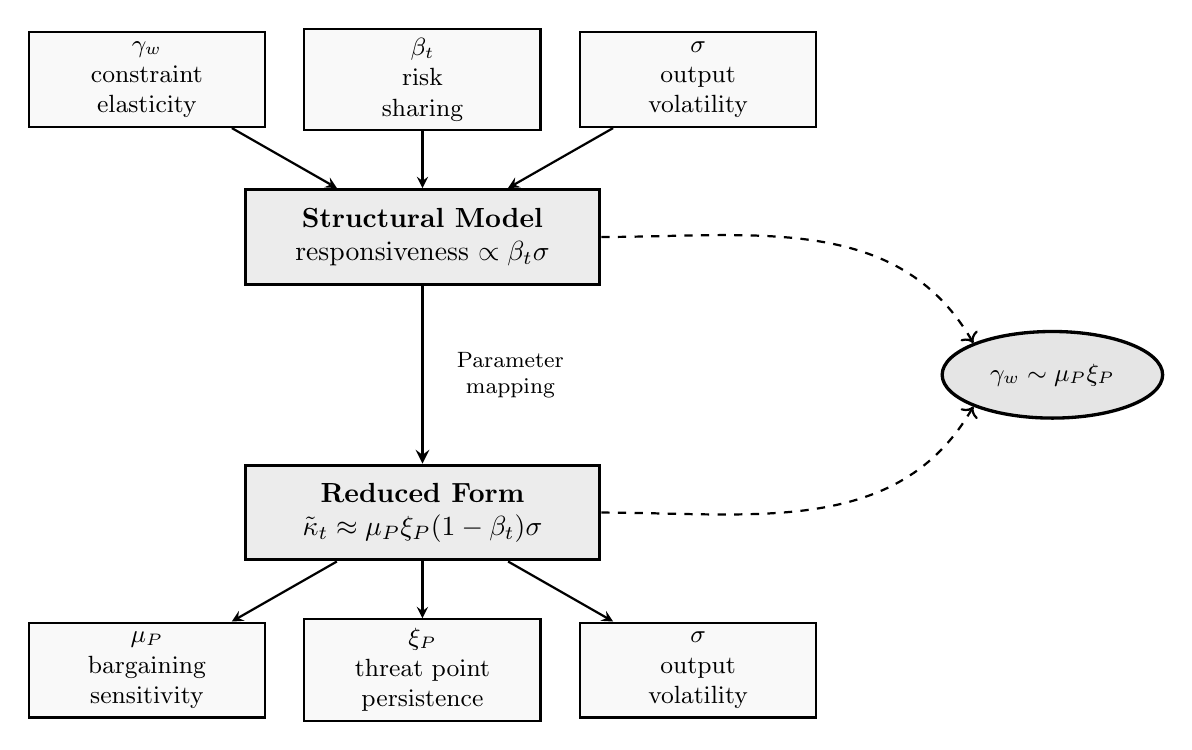
\begin{tikzpicture}[
    box/.style={rectangle, draw, thick, minimum width=3cm, minimum height=0.9cm, align=center, font=\small},
    mainbox/.style={rectangle, draw, very thick, minimum width=4.5cm, minimum height=1.2cm, align=center, font=\normalsize},
    arrow/.style={->, >=stealth, thick},
    bigarrow/.style={->, >=stealth, very thick}
]
    \node[mainbox, fill=gray!15] (structural) at (0, 2) 
        {\textbf{Structural Model}\\responsiveness $\propto \beta_t\sigma$};
    
    \node[box, fill=gray!5] (gammaw) at (-3.5, 4) 
        {$\gamma_w$\\constraint\\elasticity};
    \node[box, fill=gray!5] (beta) at (0, 4) 
        {$\beta_t$\\risk\\sharing};
    \node[box, fill=gray!5] (sigma) at (3.5, 4) 
        {$\sigma$\\output\\volatility};
    
    \draw[arrow, black] (gammaw) -- (structural);
    \draw[arrow, black] (beta) -- (structural);
    \draw[arrow, black] (sigma) -- (structural);
    
    \node[mainbox, fill=gray!15] (reduced) at (0, -1.5) 
        {\textbf{Reduced Form}\\$\tilde{\kappa}_t \approx \mu_P \xi_P (1-\beta_t) \sigma$};

    \draw[bigarrow, black] (structural) -- (reduced) 
        node[midway, right=0.3cm, align=center, font=\footnotesize, text=black] 
        {Parameter\\mapping};
        
    \node[box, fill=gray!5] (muP) at (-3.5, -3.5) 
        {$\mu_P$\\bargaining\\sensitivity};
    \node[box, fill=gray!5] (xiP) at (0, -3.5) 
        {$\xi_P$\\threat point\\persistence};
    \node[box, fill=gray!5] (sigma2) at (3.5, -3.5) 
        {$\sigma$\\output\\volatility};
    
    \draw[arrow, black] (reduced) -- (muP);
    \draw[arrow, black] (reduced) -- (xiP);
    \draw[arrow, black] (reduced) -- (sigma2);
    
    \node[draw, ellipse, very thick, fill=gray!20, minimum width=2.8cm, minimum height=1.1cm, font=\small] 
        at (8, 0.25) (equiv) {$\gamma_w \sim \mu_P \xi_P$};
    
    \draw[->, dashed, thick] (structural.east) to[out=0, in=120] (equiv.north west);
    \draw[->, dashed, thick] (reduced.east) to[out=0, in=240] (equiv.south west);
    
\end{tikzpicture}
\caption*{Source: Own elaboration.}
\label{fig:reduced_form_mapping}
\end{figure}
    
    The mapping clarifies the relationship to \textcite{digiannatale2025}. Their model specifies $\ell_{t+1} - \ell_t = \kappa \varepsilon_t$ with constant drift $\kappa$ as a primitive parameter. Our contribution is to show that this responsiveness emerges endogenously: it is proportional to $\beta_t\sigma$, with the proportionality coefficient determined by the wealth-sensitivity of the limited liability threshold through $\gamma_w$.

    %===========================================
    \section{Appendix B: Proof of Proposition \ref{prop:dynamics}} \label{ProofProp2}
    %===========================================

    We work throughout in the binding regime. Under the equilibrium contract, $y_t = \theta a_t^* + \sigma\varepsilon_t$ with $a_t^* = \beta_t^*\theta/k$, so the wealth increment satisfies
    \[
    W_{t+1} - W_t = \mu_t + \beta_t^*\sigma\varepsilon_t,
    \]
    where $\mu_t := \alpha_t^* + \beta_t^*\theta a_t^* - \frac{k}{2}(a_t^*)^2$ collects all deterministic terms. Since $\lambda_t = \lambda(W_t)$ in a PMSE and $\lambda(\cdot)$ is differentiable by assumption, a first-order Taylor expansion gives $\lambda_{t+1} - \lambda_t = \lambda'(W_t)\,\beta_t^*\sigma\varepsilon_t + o(|\varepsilon_t|)$. Applying the derivative of the logit map $d\ell/d\lambda = 1/[\lambda(1-\lambda)]$ yields the stated expansion
    \[
    \ell_{t+1} - \ell_t = \frac{\lambda'(W_t)}{\lambda_t(1-\lambda_t)}\,\beta_t^*\sigma\varepsilon_t + o(|\varepsilon_t|).
    \]
    It remains to characterize $\lambda'(W_t)$ explicitly.

    We work in the static binding regime to compute $d\beta^*/d\underline{w}$ and $d\lambda/d\underline{w}$; the dynamic case inherits the same sign structure by continuity of the continuation values in the state, as established in Proposition \ref{prop:existence}. With $\alpha = \underline{w} - \beta\underline{y}$ binding, payoffs are $\Pi(\beta) = D(\beta) + \beta\underline{y} - \underline{w}$ and $\mathrm{CE}(\beta) = C(\beta) - \beta\underline{y} + \underline{w}$. Write $\Pi_s := \Pi(\beta) - \overline{\Pi} > 0$ and $\mathrm{CE}_s := \mathrm{CE}(\beta) - \overline{\text{CE}} > 0$ for the surpluses above the respective disagreement payoffs, and $S := \Pi_s + \mathrm{CE}_s$ for total net surplus.

    Define $G(\beta,\underline{w}) := (1-\delta)\Pi'(\beta)/\Pi_s + \delta\,\mathrm{CE}'(\beta)/\mathrm{CE}_s$, where $\Pi'(\beta) = D'(\beta) + \underline{y}$ and $\mathrm{CE}'(\beta) = C'(\beta) - \underline{y}$, so that $\beta^*(W)$ satisfies $G(\beta^*,\underline{w}) = 0$. By the Implicit Function Theorem, since $\partial G/\partial\beta = \mathrm{SOC} < 0$ at the Nash optimum,
    \begin{equation}\label{eq:dbeta_dw}
    \frac{d\beta^*}{d\underline{w}} = -\frac{\partial G/\partial\underline{w}}{\mathrm{SOC}}.
    \end{equation}
    Using $\partial\Pi_s/\partial\underline{w} = -1$ and $\partial\mathrm{CE}_s/\partial\underline{w} = +1$, the numerator is
    \[
    \frac{\partial G}{\partial\underline{w}} = \frac{(1-\delta)\Pi'(\beta^*)}{\Pi_s^2} - \frac{\delta\,\mathrm{CE}'(\beta^*)}{\mathrm{CE}_s^2}.
    \]
    At the Nash optimum the FOC gives $(1-\delta)\Pi'(\beta^*)/\Pi_s = -\delta\,\mathrm{CE}'(\beta^*)/\mathrm{CE}_s$, so both terms share the same sign. Since Lemma \ref{lem:beta_bounds} established $\beta^* \in (\beta_{\min},\beta_{\max}) \subset (0,1)$ with $\mathrm{CE}'(\beta^*) < 0$, the FOC implies $\Pi'(\beta^*) > 0$, giving $\partial G/\partial\underline{w} > 0$. Together with $\mathrm{SOC} < 0$, equation \eqref{eq:dbeta_dw} yields $d\beta^*/d\underline{w} > 0$: a tighter limited liability constraint forces a higher equilibrium incentive slope.

    \textcolor{olive}{PENDIENTE: la premisa $\mathrm{CE}'(\beta^*)<0$ es falsa en la calibración base ($\mu=\theta^2/k=0.5 > \kappa=\gamma\sigma^2=0.09$, lo que da $\mathrm{CE}_t'(\beta)=(\mu-\kappa)\beta+|\underline y|>0$ para todo $\beta\ge0$, sin condición). Verificado numéricamente: en $W=0.5$, $\mathrm{CE}'(\beta^*)=+0.806$, $\Pi'(\beta^*)=-0.746$. El hecho general correcto (de la FOC, sin asumir signo) es que $\Pi'(\beta^*)$ y $\mathrm{CE}'(\beta^*)$ siempre tienen signos opuestos; aquí eso da $\partial G/\partial\underline w<0$ y por lo tanto $d\beta^*/d\underline w<0$ — signo opuesto al concluido arriba. Esto es consistente con $\beta^*(W)$ creciente en $W$ (Sección \ref{subsec:numericalresults}, confirmado con \texttt{src/model.py}: $d\beta^*/dW\approx+0.243$ en $W=0.5$). Falta rehacer esta prueba en general (casos $\mu\ge\kappa$ vs.\ $\mu<\kappa$, análogo a la Proposición de concavidad de la frontera) y propagar el signo correcto a la Ecuación \eqref{eq:dlambda_dw}, la condición \eqref{eq:lambda_sign_condition}, el Teorema \ref{thm:central}, y la Figura \ref{fig:wealth_dynamics}.}

    Differentiating $\lambda = \mathrm{CE}_s/S$ with respect to $\underline{w}$, accounting for both the direct and indirect effects through $\beta^*$, gives
    \[
    \frac{d\lambda}{d\underline{w}} = \frac{1}{S} + \frac{d\beta^*}{d\underline{w}} \cdot \frac{\mathrm{CE}'(\beta^*)S - \mathrm{CE}_s\,S'(\beta^*)}{S^2}.
    \]
    Substituting $\Pi'(\beta^*) = -\frac{\delta}{1-\delta}\frac{\Pi_s}{\mathrm{CE}_s}\mathrm{CE}'(\beta^*)$ from the Nash FOC, the numerator of the second term simplifies to $\mathrm{CE}'(\beta^*)[\Pi_s + \frac{\delta}{1-\delta}\mathrm{CE}_s]$. Since $\mathrm{CE}'(\beta^*) < 0$ and the bracket is strictly positive, the second term is negative, giving
    \begin{equation}\label{eq:dlambda_dw}
    \frac{d\lambda}{d\underline{w}} = \frac{1}{S} - \frac{d\beta^*}{d\underline{w}} \ \frac{|\mathrm{CE}'(\beta^*)|}{S^2}\left[\Pi_s + \frac{\delta}{1-\delta}\mathrm{CE}_s\right].
    \end{equation}
    The first term is the direct transfer effect: tightening the constraint shifts one unit of surplus to the agent. The second term is the indirect incentive effect: the forced increase in $\beta^*$ raises the agent's risk exposure, partially offsetting the direct gain.

    From \eqref{eq:dlambda_dw}, $d\lambda/d\underline{w} < 0$, equivalently $\lambda'(W) > 0$, if and only if
    \begin{equation}\label{eq:lambda_sign_condition}
    \frac{d\beta^*}{d\underline{w}} \cdot |\mathrm{CE}'(\beta^*)| \cdot \left[\Pi_s + \frac{\delta}{1-\delta}\mathrm{CE}_s\right] < 1.
    \end{equation}
    The left side measures how much the agent's certainty equivalent falls per unit increase in $\underline{w}$ through the forced increase in $\beta^*$, weighted by the agent's relative stake $(1-\delta)^{-1}$. The condition holds generically: it is satisfied whenever the Nash FOC is steep at $\beta^*$ (large $|\mathrm{SOC}|$) or whenever $\beta^*$ is close to $\beta^{\mathrm{eff}}$ so that $|\mathrm{CE}'(\beta^*)|$ is small. The dynamic case inherits the sign by continuity of $V_A^b(W;\beta)$ in $\mathrm{CE}(\beta)$ on $\mathcal{S}$, with the argument unchanged upon replacing $\mathrm{CE}_s$ by $V_A^b - \overline{\text{CE}}$.

    The chain rule then gives $\lambda'(W) = (-\gamma_w)(d\lambda/d\underline{w})$. Under condition \eqref{eq:lambda_sign_condition}, $d\lambda/d\underline{w} < 0$, so $\lambda'(W) > 0$: bargaining power is strictly increasing in accumulated wealth in the binding regime, with magnitude proportional to $\gamma_w$. When $\gamma_w = 0$ the mechanism shuts down. In the slack regime $\lambda_t = \delta$ for all $W_t$, so $\lambda'(W_t) = 0$ and $\ell_t$ is constant. \qed

    %===========================================
    \section{Appendix C: Proof of Proposition \ref{prop:ergodic}} \label{ProofProp3}
    %===========================================

    We first establish that the equilibrium slope is bounded away from zero and one on the binding domain, then use this bound in a Foster-Lyapunov argument to prove geometric ergodicity.

    \begin{lemma}[Boundedness of equilibrium slope]\label{lem:beta_bounds}
    Let $\mathcal{W} := \{W \geq 0 : \underline{w}(W) > \underline{w}^{\,\mathrm{slack}}\}$ be the binding domain, where $\underline{w}^{\,\mathrm{slack}}$ is the limited liability floor at which the unconstrained Nash solution exactly satisfies limited liability. On $\mathcal{W}$, the equilibrium slope satisfies $\beta^*(W) \in [\beta_{\min}, \beta_{\max}]$ for constants $0 < \beta_{\min} \leq \beta_{\max} < 1$.
    \end{lemma}

    \begin{proof}
    Define $F(\beta, W) := (1-\delta)\,\frac{\partial}{\partial\beta} V_P^b(W;\beta)\,/\,[V_P^b(W;\beta) - \overline{\Pi}] + \delta\,\frac{\partial}{\partial\beta} V_A^b(W;\beta)\,/\,[V_A^b(W;\beta) - \overline{\text{CE}}]$, so that $\beta^*(W)$ satisfies $F(\beta^*(W), W) = 0$.

    At $\beta = 0$: increasing $\beta$ raises induced effort $a^* = \beta\theta/k$ from zero, which strictly increases expected output and hence $V_P^b$. Since $V_P^b(W;0) - \overline{\Pi} > 0$ by individual rationality, the first term of $F$ is strictly positive. The second term is finite. Hence $F(0, W) > 0$.

    At $\beta = 1$: the agent bears full output risk. The risk premium is $(\gamma/2)\sigma^2$, while the marginal benefit of raising $\beta$ toward 1 in terms of effort is $\theta^2/k$. The condition $\beta^{\mathrm{eff}} < 1$, which holds whenever $\gamma\sigma^2 > 0$ and $\theta, k$ are finite, implies that the total surplus $S(\beta)$ is strictly decreasing at $\beta = 1$. It follows that $\frac{\partial}{\partial\beta} V_A^b(W;1) < 0$ and the second term of $F$ dominates, giving $F(1, W) < 0$.

    Since $F(\cdot, W)$ is continuous on $[0,1]$ and changes sign, the intermediate value theorem yields at least one solution $\beta^*(W) \in (0,1)$. The second-order condition of the Nash problem ensures the solution is locally unique. Since period payoffs and continuation values are continuous and bounded on $\mathcal{S}$ (Assumption \ref{ass:compact_domain}), $F(\beta, W)$ is uniformly equicontinuous in $(\beta, W)$ on $[0,1] \times \mathcal{W}$. The solution correspondence is therefore upper hemicontinuous with nonempty values in $(0,1)$. On a compact domain, the image of a compact set under an upper hemicontinuous correspondence with closed values is compact, so $\beta^*(W)$ attains values in a closed subset $[\beta_{\min}, \beta_{\max}] \subset (0,1)$.
    \end{proof}

    \begin{proof}[Proof of Proposition \ref{prop:ergodic}]
    We apply the Foster-Lyapunov drift criterion for geometric ergodicity \parencite[Theorem 15.2.5]{meyn2009}. Let $\mathcal{V}(W) = W^2$ serve as the Lyapunov function. We must exhibit constants $c \in (0,1)$ and $b < \infty$ such that
    \begin{equation}\label{eq:fl}
        \mathbb{E}[\mathcal{V}(W_{t+1}) \mid W_t = W] \leq (1-c)\,\mathcal{V}(W) + b \qquad \text{for all } W \geq 0.
    \end{equation}

    In the binding regime, $\alpha^*(W) = \overline{w} - \gamma_w W - \beta^*(W)\underline{y}$, so with $a^* = \beta^*(W)\theta/k$ and $y_t = \theta a^* + \sigma\varepsilon_t$ the wealth update takes the form $W_{t+1} = W + \mu(W) + \beta^*(W)\sigma\varepsilon_t$, where the deterministic drift is $\mu(W) := \overline{w} - \gamma_w W - \beta^*(W)\underline{y} + [\beta^*(W)]^2\theta^2/(2k)$. By Lemma \ref{lem:beta_bounds}, $\beta^*(W) \leq \beta_{\max}$ on $\mathcal{W}$. Setting $K_1 := \beta_{\max}^2\theta^2/(2k)$, $K_2 := \beta_{\max}|\underline{y}|$, and $A := \overline{w} + K_1 + K_2$, we have $\mu(W) \leq A - \gamma_w W$ for all $W \in \mathcal{W}$. In the slack regime the agent accumulates at most $S^{\mathrm{eff}}$ per period net of effort costs, so by enlarging $A$ if necessary the same bound holds uniformly across both regimes.

    Since $\varepsilon_t \sim \mathcal{N}(0,1)$ is independent of $W_t$, the conditional second moment satisfies $\mathbb{E}[W_{t+1}^2 \mid W_t = W] = (W + \mu(W))^2 + [\beta^*(W)]^2\sigma^2$, and therefore
    \[
    \mathbb{E}[\mathcal{V}(W_{t+1}) \mid W_t = W] - \mathcal{V}(W) = 2W\mu(W) + \mu(W)^2 + [\beta^*(W)]^2\sigma^2.
    \]
    Applying $\mu(W) \leq A - \gamma_w W$ to each term: $2W\mu(W) \leq 2AW - 2\gamma_w W^2$, $\mu(W)^2 \leq 2A^2 + 2\gamma_w^2 W^2$, and $[\beta^*(W)]^2\sigma^2 \leq \beta_{\max}^2\sigma^2$. Summing these bounds gives
    \[
    \mathbb{E}[\mathcal{V}(W_{t+1}) \mid W_t = W] - \mathcal{V}(W) \leq -2\gamma_w(1-\gamma_w)W^2 + 2AW + 2A^2 + \beta_{\max}^2\sigma^2.
    \]
    The coefficient on $W^2$ is $-2\gamma_w(1-\gamma_w)$, which is strictly negative under the assumption $\gamma_w \in (0,1)$. Setting $c_0 := 2\gamma_w(1-\gamma_w) > 0$, the right-hand side is a concave quadratic in $W$ bounded above, so for any $c \in (0,c_0)$ there exists a finite $b$ such that $-c_0 W^2 + 2AW + 2A^2 + \beta_{\max}^2\sigma^2 \leq -cW^2 + b$ for all $W \geq 0$. This establishes \eqref{eq:fl}.

    To complete the argument, note that the full-support Gaussian innovation implies $W_{t+1} = W + \mu(W) + \beta^*(W)\sigma\varepsilon_t$ assigns positive probability to every open interval from any starting point $W \geq 0$, so the chain is irreducible with respect to Lebesgue measure on $[\underline{W},\infty)$ and aperiodic. The Foster-Lyapunov condition \eqref{eq:fl} together with irreducibility and aperiodicity implies geometric ergodicity by \parencite[Theorem 15.2.5]{meyn2009}. Existence and uniqueness of $\Phi^*$ follow from the same theorem.
    \end{proof}

\end{appendices}

\end{spacing}
\end{document}